\chapter{MixedAim: The Mixed-Initiative System}

MixedAim is the tool we developed with which designers can interactively design PuzzleScript levels. The binaries and source code for MixedAim is published at \url{https://dekeyser.ch/mixedaim}.

\section{PuzzleScript}

The programming language with which designers can implement puzzle games in MixedAim is \href{https://www.puzzlescript.net}{PuzzleScript}\footnote{\url{https://www.puzzlescript.net} @ PuzzleScript} developed by Stephen Lavelle (also known as increpare).
In the appendix \autoref{fig:sokobaninpuzzlescript}, we have published a full Sokoban implementation in PuzzleScript for reference.

PuzzleScript is grid-based, and each PuzzleScript game consists out of the following seven sections.
\begin{description}
    \item[Objects] In here, the objects of the grid and their style are declared. For Sokoban, one would have to declare the following objects \textit{Background, Walls, Player, Crate, Target}. \textit{Player} and \textit{Background} are special objects and always need to be declared. \hfill
        \begin{figure}[!htbp]
    \begin{minipage}{0.4\textwidth}
        \centering
    \begin{lstlisting}
========
OBJECTS
========
Wall
BROWN DARKBROWN
00010
11111
01000
11111
00010
    \end{lstlisting}
    
    \end{minipage} \qquad $\Longrightarrow$ \hfill
    \begin{minipage}{0.4\textwidth}
        
        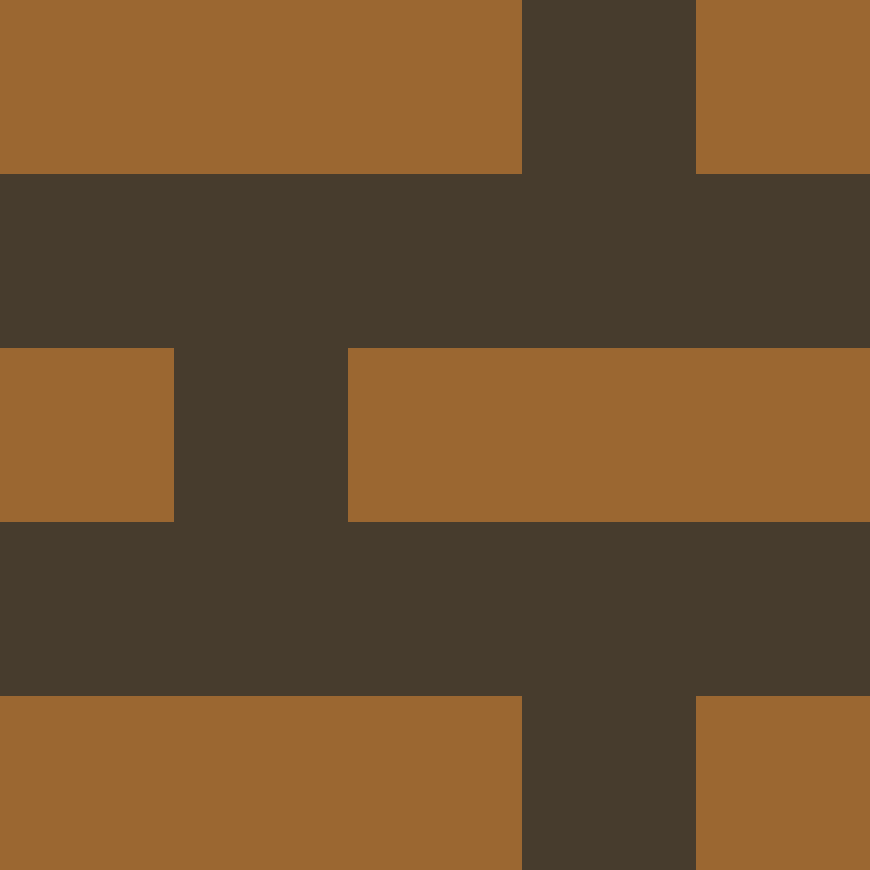
\includegraphics[width=0.55\textwidth]{figures/wallimg.png}
    \end{minipage}
    \caption{Objects section}
    \end{figure}



    \item[Legend] In the legend,  three kinds of names can be specified.
        \begin{enumerate}
            \item Define a synonym for an object. \hfill \\
            Example: \lstinline{# = Background}
            \item Define an aggregate, which is a symbol for referencing a tile that includes multiple objects. It is not possible to create an aggregate from objects which belong to the same collision layer. \hfill \\
            Example: \lstinline{@ = Target and Background}
            \item Define a property, which references any tile that contains any of the objects included in its definition. \hfill \\
            Example: \lstinline{Obstacle = Wall or Crate or Player or Target}.
        \end{enumerate}
        
        It is worth mentioning that it is not possible to define aggregates from properties or vice-versa.
    
    
    \item[Sounds] can be used to add chip-tunes generated with \href{https://www.bfxr.net}{Bfxr} \footnote{\url{https://www.bfxr.net}}.
    
    \item[Collisionlayers] define on which layer which objects are stored. In PuzzleScript a level is rendered by multiple two-dimensional layers layered on top of each other.
     In this way one can specify that both a \textit{Player} and a \textit{Wall} cannot both occupy the same tile while a \textit{Crate} and a \textit{Target} can.
     
             \begin{figure}[!htbp]
    \begin{minipage}{0.4\textwidth}
        \centering
    \begin{lstlisting}
================
COLLISIONLAYERS
================
Background
Target
Player"Wall"Crate
    \end{lstlisting}
    
    \end{minipage} \qquad $\Longrightarrow$ \hfill
    \begin{minipage}{0.45\textwidth}
    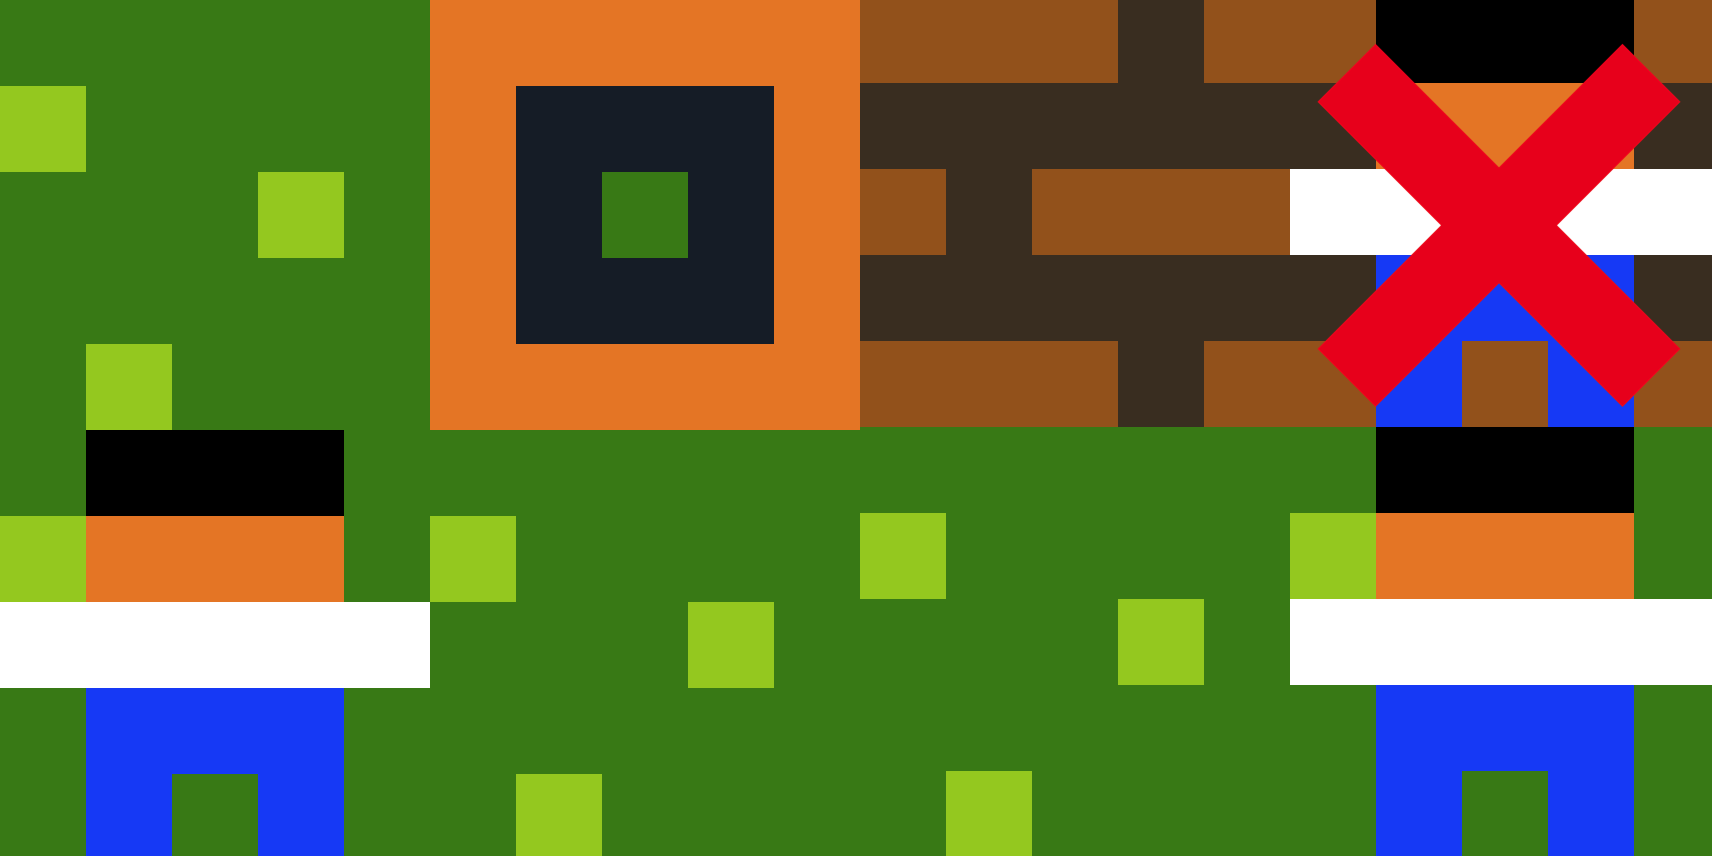
\includegraphics[width=0.7\textwidth]{figures/collisionlayersboth.png}
    \end{minipage}
    \caption{Collisionlayers section}
    \end{figure}
    
    \item[Rules] The rules are deceptively simple and are structured in the following form \: \lstinline{Match -> Replace}. \textit{Match} consists of either rows or columns that have to be matched and \textit{Replace} must be of the same size stating with what the objects will be replaced.
        
    Every object can come with force attached to it (highlighted in green by the examples). Forces are used to record player inputs. When the player presses the right button, all \textit{Player} objects get the right force assigned to them. In the end, when all (non-late) rules have been applied, each object will try to move in the direction of their force. This will succeed provided there is no object of the same collision layer in that direction.
        
        The rules of Sokoban can be written with a single rule: \hfill \\
        \lstinline{[> Player | Crate] -> [ > Player | > Crate ]}
        
        This rule is implicitly expanded in 4 directions, so it works both on columns and rows:\hfill \\
        \lstinline{RIGHT  [right Player | Crate] -> [right Player | right Crate]}\hfill \\
        \lstinline{+ UP   [up    Player | Crate] -> [up    Player | up    Crate]}\hfill \\
        \lstinline{+ DOWN [down  Player | Crate] -> [down  Player | down  Crate]}\hfill \\
        \lstinline{+ LEFT [left  Player | Crate] -> [left  Player | left  Crate]}\hfill \\
        
        To match multiple rows/columns at once, one can use multiple boxes. Take the following rule as an example. If the player is on top of a key and there is a door on the map, then remove the key and the door.
    \lstinline{[Player Key] [Door] -> [Player] []}
    
        Lastly, every command can execute \textit{commands} if the rule is executed, such as playing a tune defined in the sound section, stopping the current moves (\textit{cancel}), replaying the rules another time (\textit{again}) \& more.
        
        Additionally, one can use properties and aggregates within rules, use the keyword \textit{No} to make sure no object/aggregate/property matches, use an ellipsis for arbitrary distances, build groups of rules, make these groups rigid \& a lot more.
        
        For more details please consult the \href{https://www.puzzlescript.net}{PuzzleScript manual}\footnote{\url{https://www.puzzlescript.net} @ PuzzleScript}.
        
        We also linked a BNF grammar for a single syntactically correct PuzzleScript rule (without rule grouping) \ref{fig:puzzlescriptrulebnf}.
    
    \item [Winconditions] In this section, one can add multiple win-conditions which all need to be satisfied in the level state simultaneously to `win' a level.
    
    The rules can be any of the following: \textit{No X, Some X, No X on Y, Some X on Y, All X on Y} where X and Y can be objects or properties and do what one would expect them to do.
    
    \item[Levels] is the section where one can specify the puzzle problems, also referred to as levels.
    The previously defined objects/synonyms/aggregates with a single letter can be used to create the level.
            \begin{figure}[!htbp]
    \begin{minipage}{0.4\textwidth}
        \centering
    \begin{lstlisting}
========
LEVELS
========
####..
#.O#..
#..###
#@P..#
#..*.#
#..###
####..
    \end{lstlisting}
    
    \end{minipage} \qquad $\Longrightarrow$ \hfill
    \begin{minipage}{0.4\textwidth}
        
        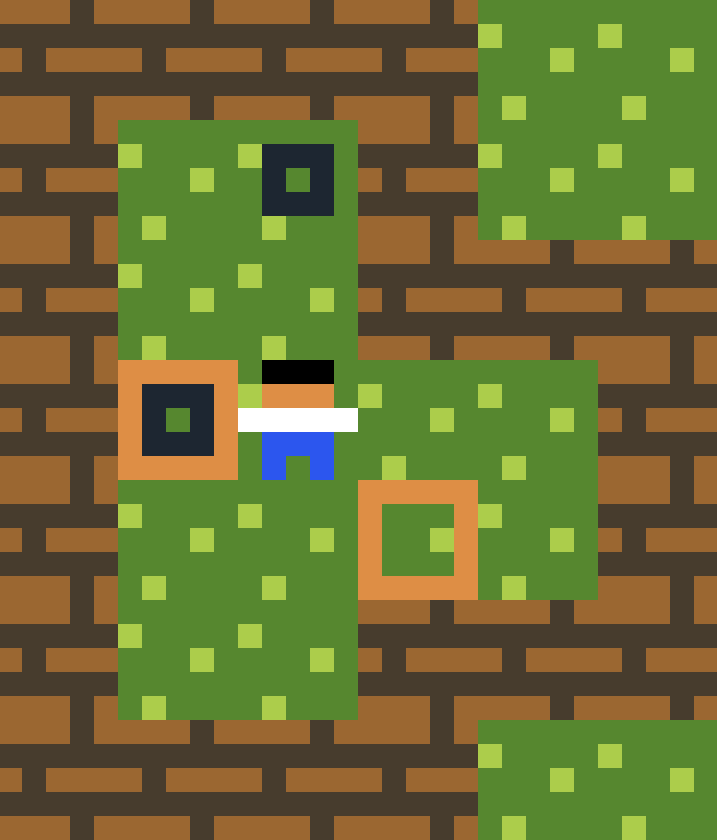
\includegraphics[width=0.55\textwidth]{figures/level1.png}
    \end{minipage}
    \caption{Levels section}
    \end{figure}
     
\end{description}


\section{User interface}

The mixed-initiative system we developed to create PuzzleScript levels is comprised of three modes of operation: The \textit{level editor mode} [\autoref{fig:leveleditormode}], where the designer can place the blocks on the level, the \textit{playtest mode} [\autoref{fig:playtestmode}], where the player can test the level and see if it is solvable from a certain position and lastly the \textit{transform mode} [\autoref{fig:transformermode}], where the designers can steer the passive suggestions which are shown both in the \textit{level editor} and in the \textit{transform mode}.

%   a level they are working on in order to see possible variations of the design and get inspired by them.

% \cite{Lawson1997} roles for the mixed initiative system are as follows.
\begin{figure}
\centering
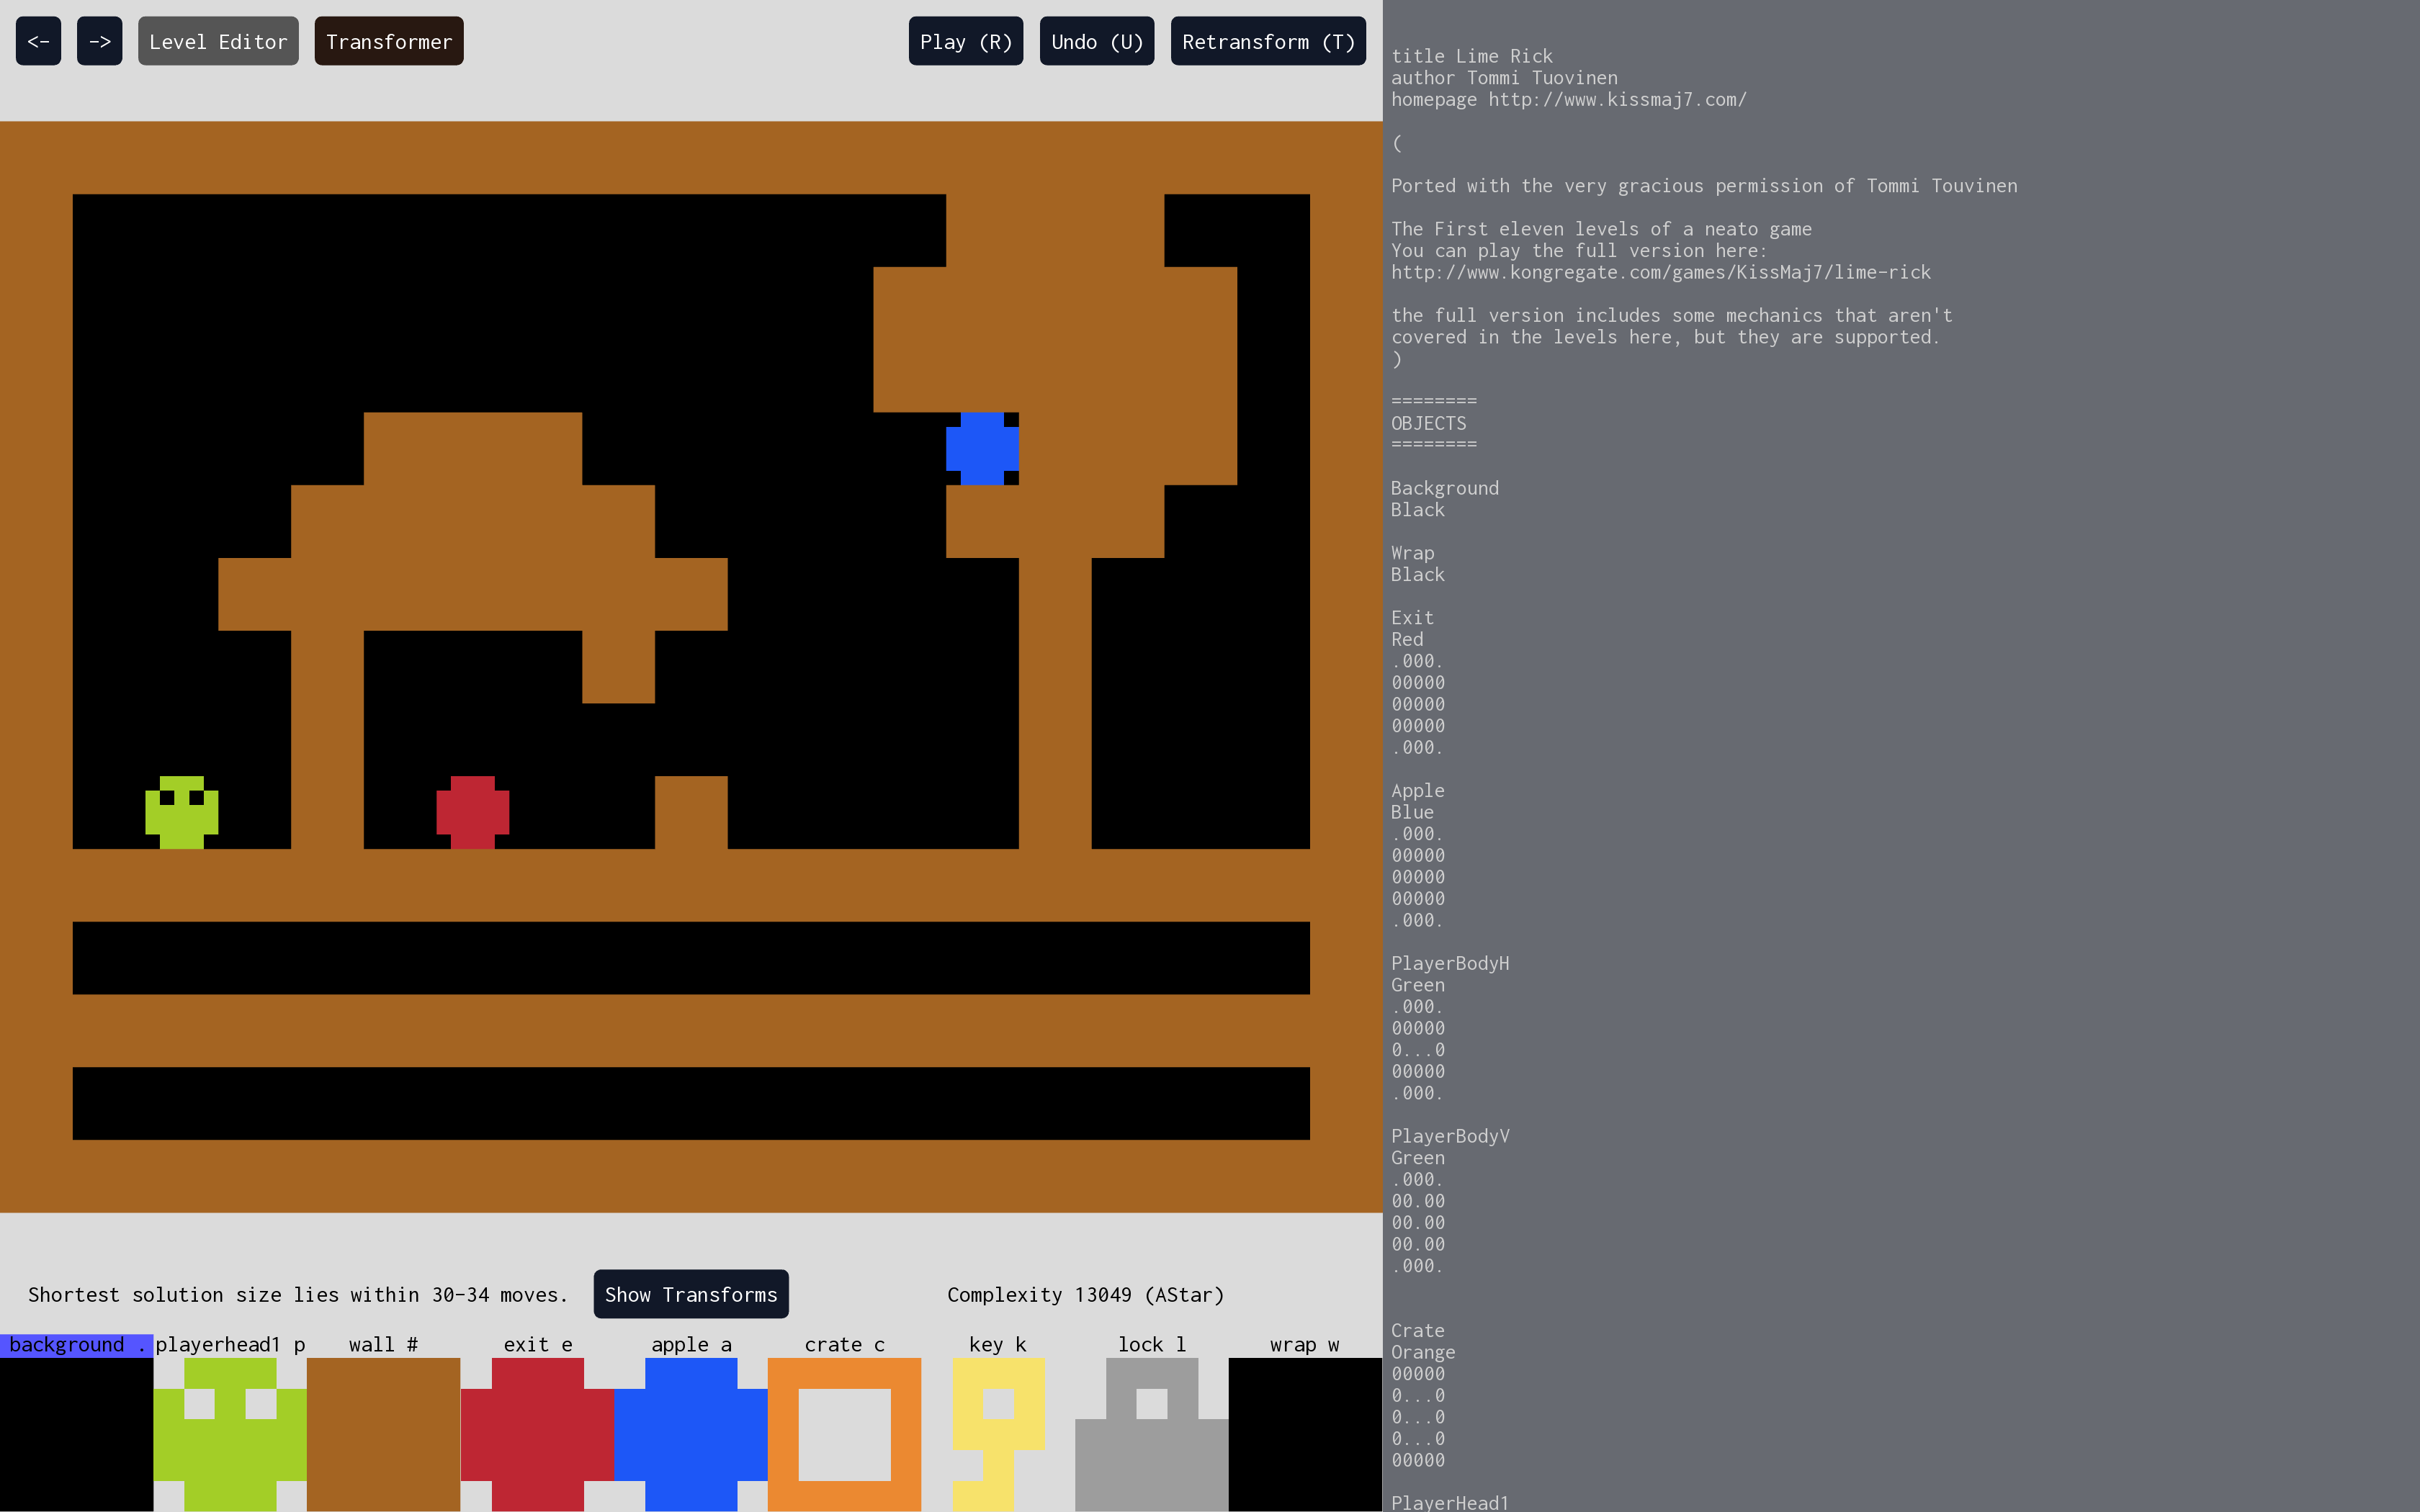
\includegraphics[width=1.0\linewidth]{figures/leveleditormode.png}
\caption[LevelEditor]{Level Editor Mode\label{fig:leveleditormode}}
\end{figure}


\begin{figure}
\centering
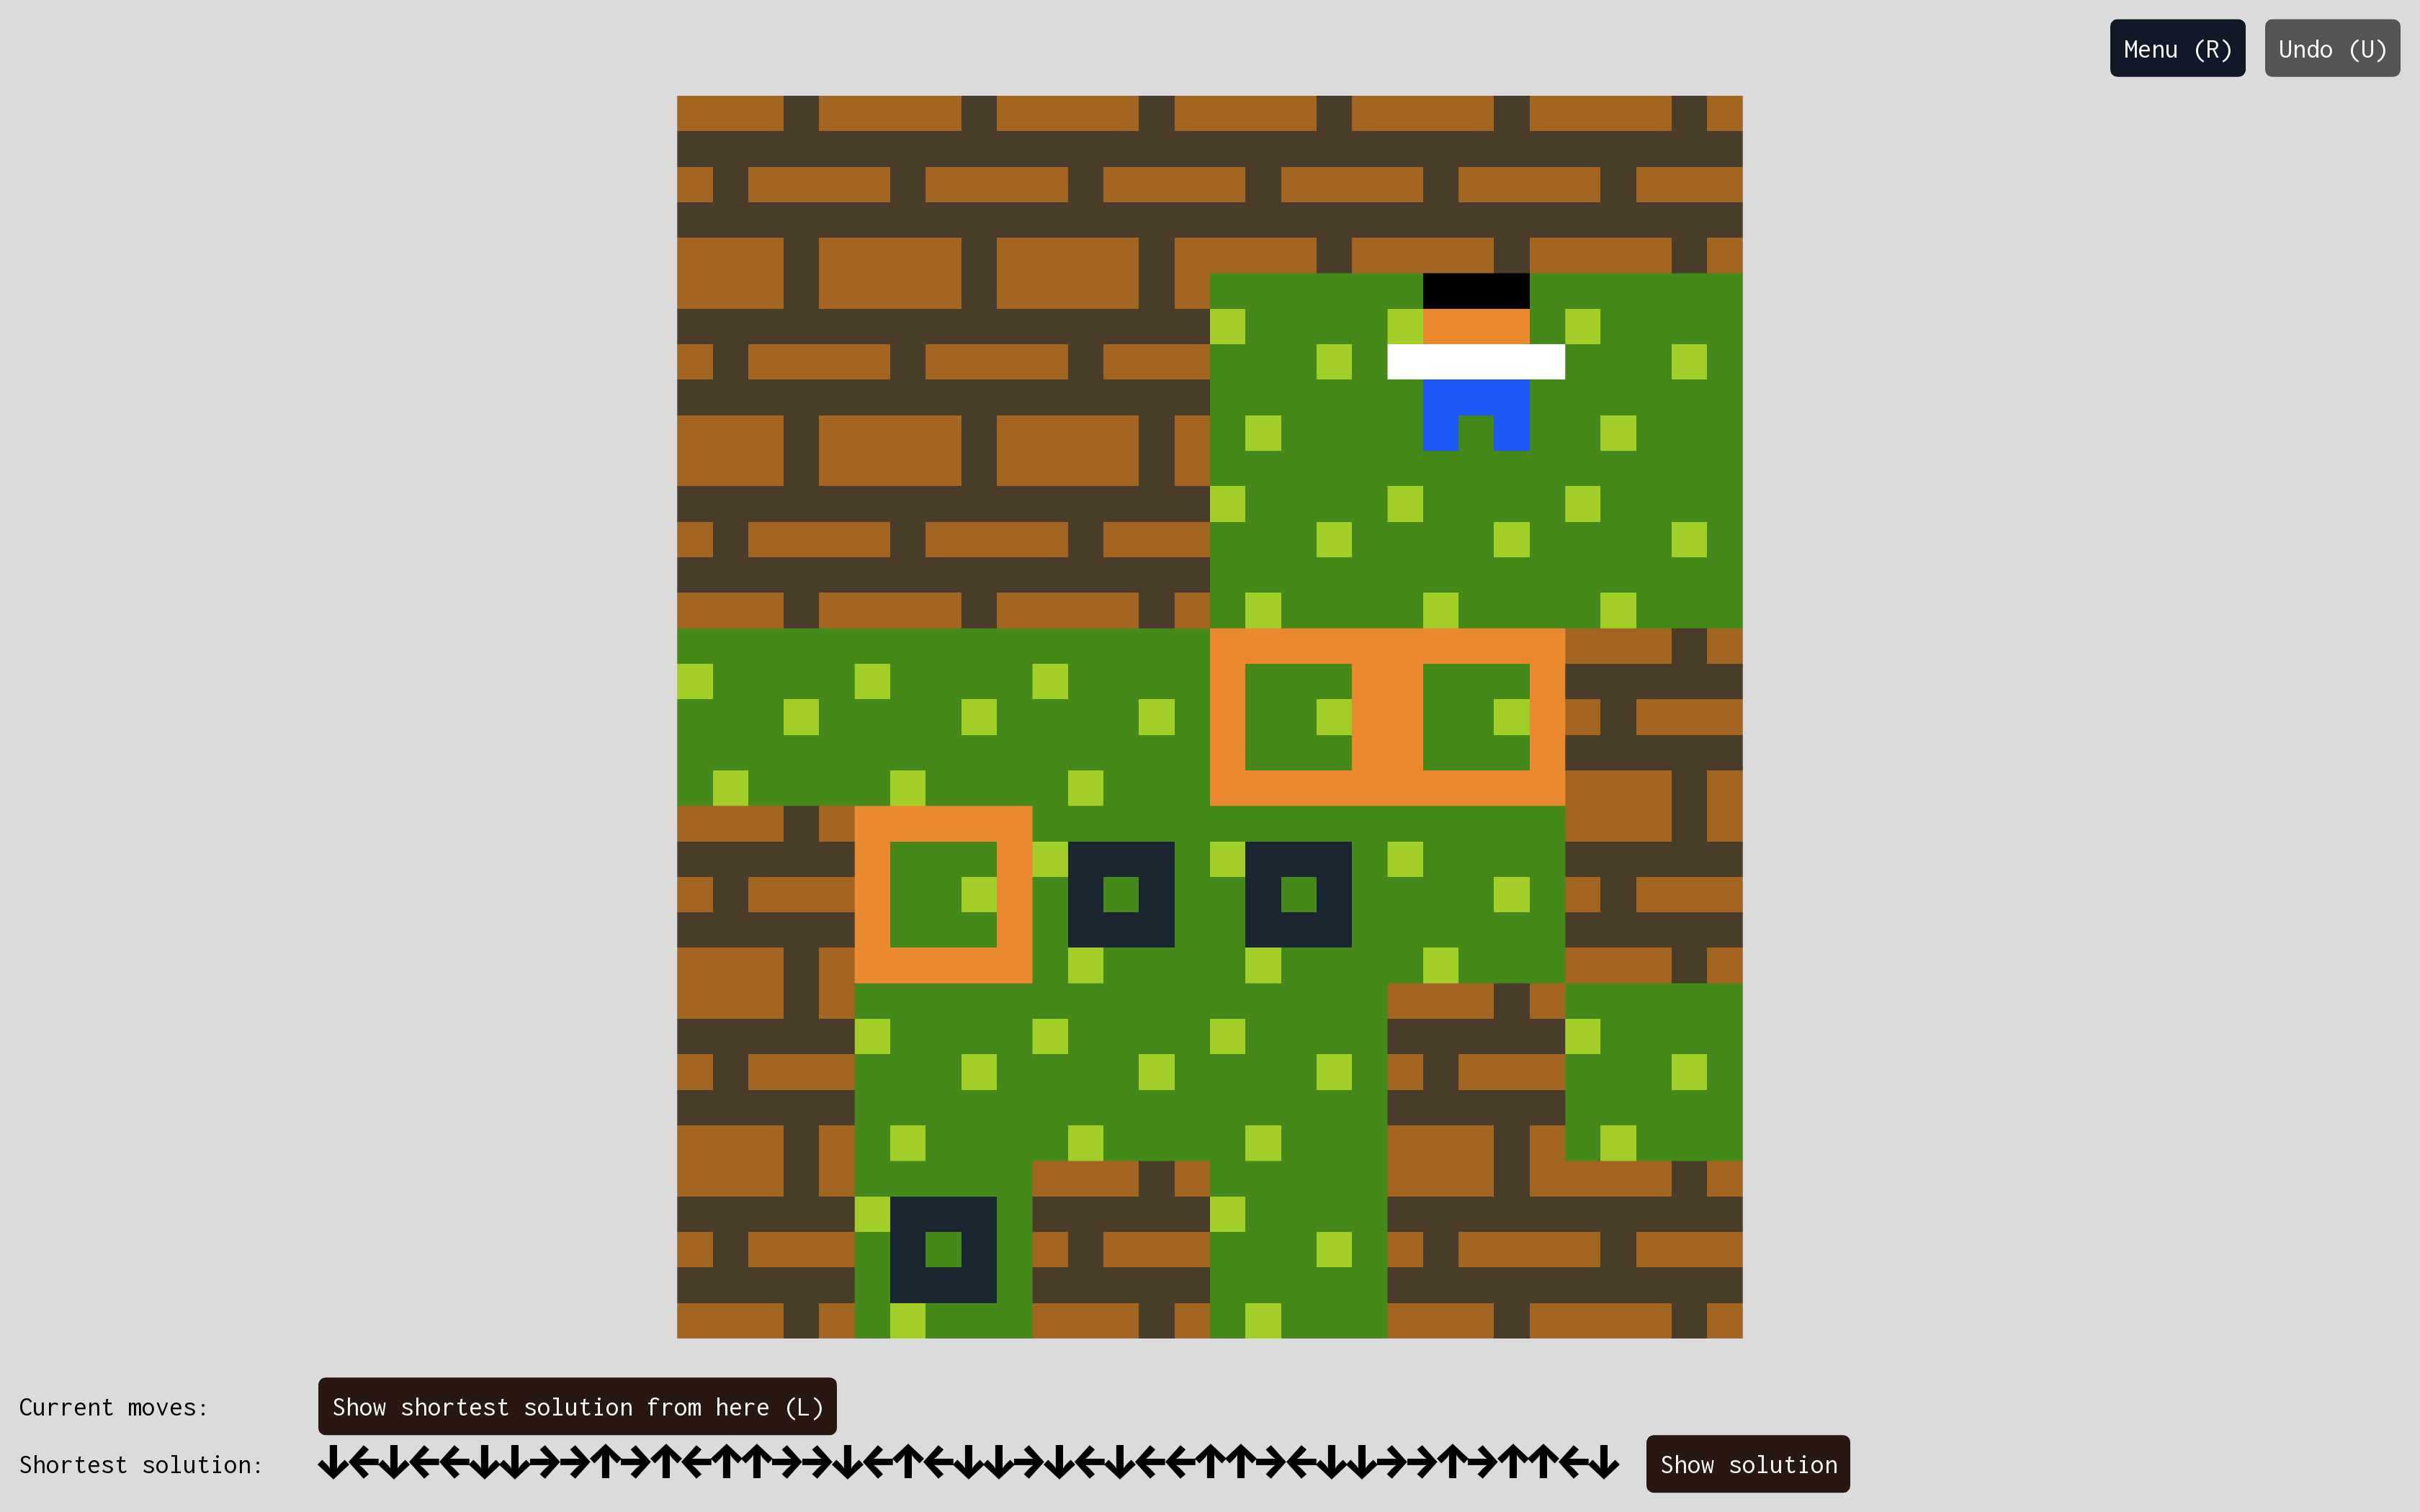
\includegraphics[width=1.0\linewidth]{figures/playtestmode.png}
\caption[Playtest]{Playtest Mode\label{fig:playtestmode}}
\end{figure}

\begin{figure}
\centering
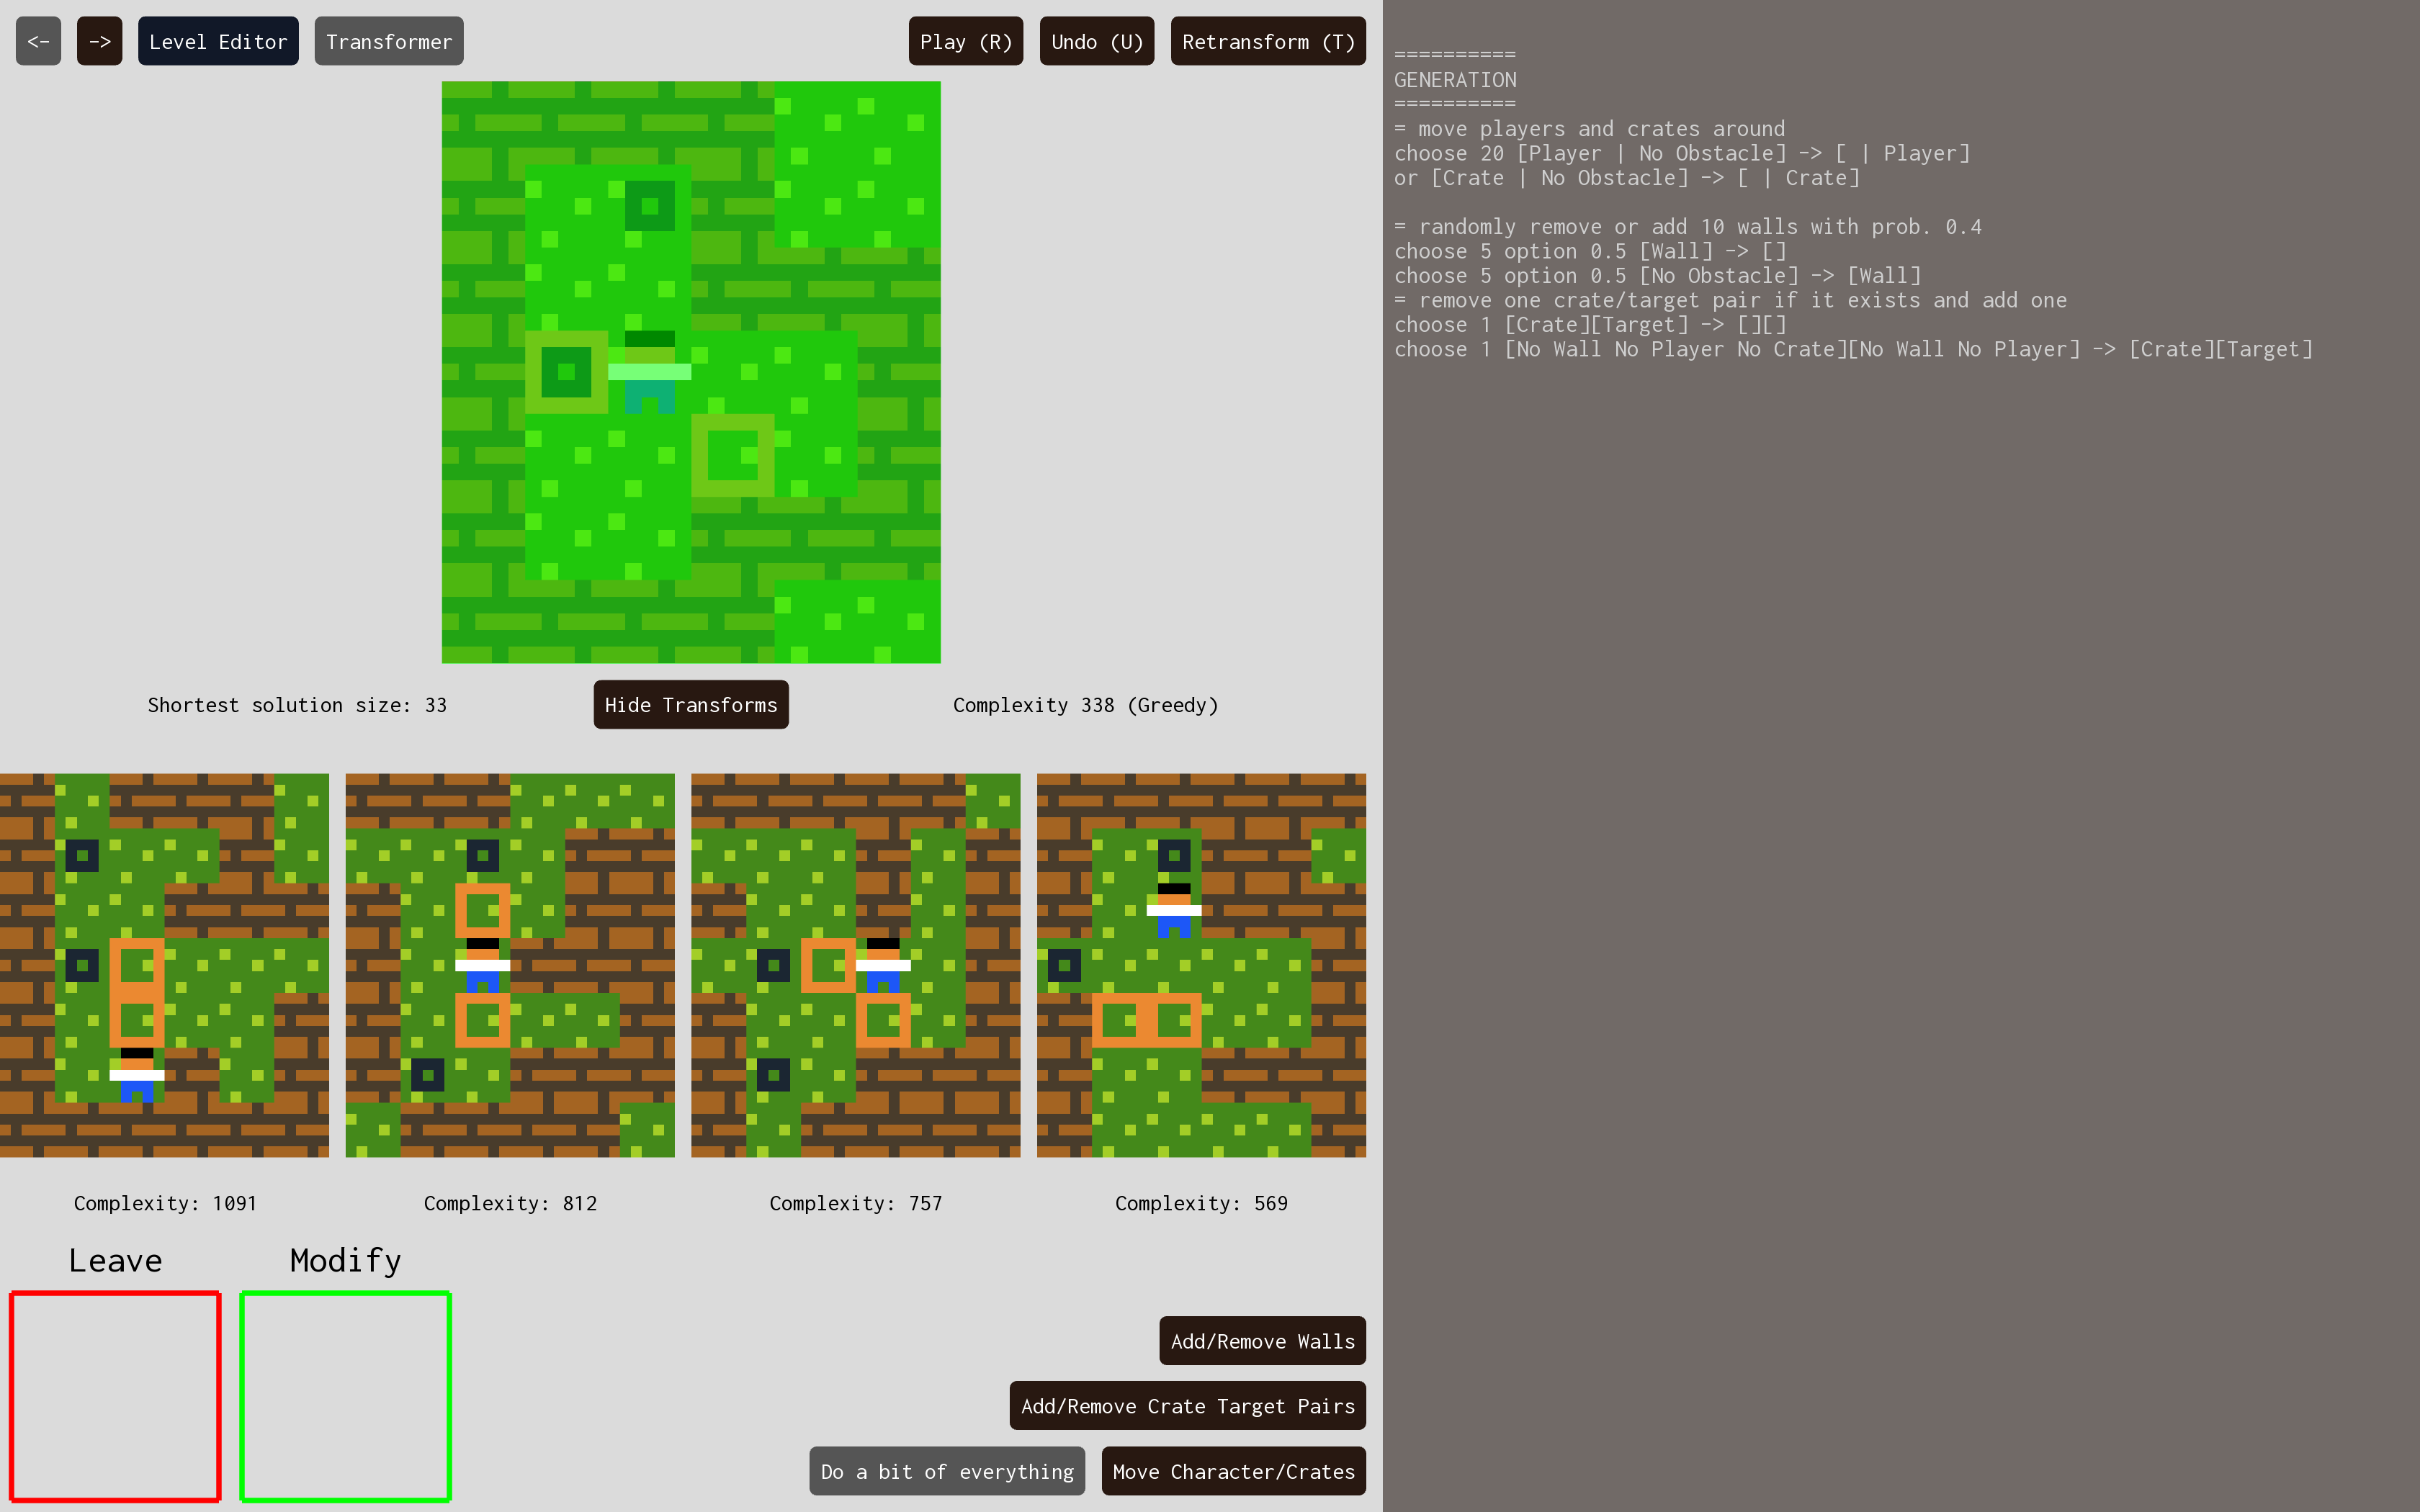
\includegraphics[width=1.0\linewidth]{figures/imageoftransformmode.png}
\caption[Transformer]{Transform Mode\label{fig:transformermode}}
\end{figure}

Information about the current level is passively shown at all times to the designer [\autoref{fig:passiveinformation}] and includes information like whether or not a level is solvable, and, if it is, in how many steps at least. Additionally, it also displays the difficulty of the level.
This allows designers to quickly see whether a modification on a level they are working on is still solvable without needing to solve it themselves. In the next chapter, we will discuss in which ways designers exploit this when designing a level.


\begin{figure}
\centering
\hfill
\begin{minipage}[t][5cm][b]{0.35\textwidth}
\centering

\includegraphics[width=1.0\linewidth]{figures/shortestsolution.png} \hfill

\includegraphics[width=1.0\linewidth]{figures/shortestsolutionwithin.png}\hfill

\includegraphics[width=1.0\linewidth]{figures/nosolutionwithin.png}\hfill
Solve Information
\label{fig:solveinformation}
%\caption{Solve \\ Information}
\end{minipage}
\begin{minipage}[t][5cm][b]{0.25\textwidth}
\centering
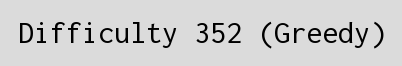
\includegraphics[width=1.0\linewidth]{figures/difficultygreedy.png}\hfill
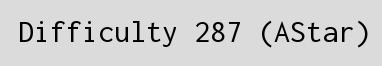
\includegraphics[width=1.0\linewidth]{figures/difficultyastar.png}\hfill

\includegraphics[width=1.0\linewidth]{figures/difficultybfs.png}\hfill
\label{fig:solveinformation}
Difficulty Information
%\caption{Difficulty Information}
\end{minipage}
\begin{minipage}[t][5cm][b]{0.35\textwidth}
\centering
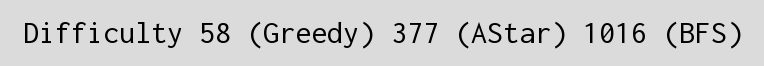
\includegraphics[width=1.0\linewidth]{figures/difficultycurveleft.png} \hfill

\includegraphics[width=1.0\linewidth]{figures/difficultycurveright.png}\hfill
\label{fig:solveinformation}
Greedy vs. AStar vs. BFS
%\caption{Greedy vs. AStar vs. BFS}
\end{minipage}


\caption{Passive information displayed to the user\label{fig:passiveinformation}}
\end{figure}


\section{Solver \& Difficulty}
To check solvability, we employ three different types of solver: Breadth-first search, A* search, and Greedy best-first search. All of these search algorithms are complete, meaning they will find a solution eventually since the search state space of PuzzleScript is finite. The breadth-first search algorithm guarantees to find the smallest solution but is often too slow due to the size of the PuzzleScript state space.

Both A* and Greedy search need a heuristic which, given a state, approximates the number of steps the state is away from a solution. Ideally, this heuristic never overestimates the number of steps, making it admissible \ref{eq:admissibility}. That way any solution found by A* will, like breadth-first search, require the least number of moves. If we only care about finding any solution, the greedy best-first search usually is the fastest.

\begin{equation}
\label{eq:admissibility}
\forall s_i \in \text{STATES} \: . \: h(s_i) \leq \text{min-cost-to-goal-from}(s_i)
\end{equation}

It is a popular misconception that A* performs optimally under a heuristic $h$, in the sense that it expands the fewest number of nodes, compared to other search algorithms that also only rely on $h$ and only search from the start. \cite{Holte2010} elaborates this in more detail, but this is not true if we store which nodes were already expanded (referred to as a closed set). In many puzzle games, like Sokoban, it is possible to end up in the same state via multiple paths. For example, moving up or moving left, up, right leads to the same state if no obstacles block the path. This might lead A* to reopen a state.
If $h$ additionally is consistent/monotone \ref{eq:monotone} however, then this claim is valid because A* does not need to re-evaluate already visited states / states in the closed set.     

\begin{equation}
\label{eq:monotone}
\forall n_i \in \text{NEIGHBOR}(s_i) \: . \: h(s_i) \leq d(s_i, n_i) + h(n_i)
\end{equation}

Notice that not all puzzles profit from carrying a closed set. For example, it is not possible to reach the same state via different paths in a puzzle where one moves an ever-expanding snake. In this case, keeping a closed set is just a memory overhead.
Further techniques like iterative deepening A* have been employed to address the cost of keeping such a closed set, but we have not implemented these methods.

In practice, the greedy best-first search outperforms A* in many cases and BFS in some other cases (tested games include Sokoban, LimeRick, Sokobond). When Greedy performs better than A*, then usually BFS performs even worse and when BFS performs better than A* then usually Greedy performs even worse making A* our default solver for the suggestions (see next section). 

The heuristic we use for the A* and Greedy solver is a generalized version of \cite{Junghanns1999} Sokoban heuristic. Since every crate has to be pushed on a target (and two crates cannot be on the same target) Junghanns observes that the minimal matching between crates and targets (the cost of matching a pair being the Manhatten distance) is an admissible heuristic for Sokoban.

The win-condition of Sokoban implemented in PuzzleScript is: \lstinline{All Crate on Target}. Notice that there can be more targets than crates, so we want to find the minimal-cost maximum matching.

\hspace{\dimexpr-\fboxrule-\fboxsep\relax}\fbox{%
  \begin{minipage}[t]{\textwidth}
A PuzzleScript file can contain multiple win-conditions that all need to be satisfied. We compute the heuristic $h(s)$ for state $s$ as the sum of all of the following win-conditions:  \hfill      \begin{description}
\item[No X:] As soon as X is nowhere on the level state this win-condition is triggered. We add +1 cost for every X appearing on the state s.
\item[Some X:] As soon as X is somewhere on the level state this win-condition is triggered. We add +1 cost if no X is found in the state s.    

\item[No X on Y:] We add +1 for every tile that has both X and Y on it.
\item[Some X on Y:] We compute the closest $X,Y$ pair in terms of their Manhattan distance and add their distance towards the cost function.
\item[All X on Y:] We compute the minimal-cost maximum matching on the Manhattan distance of all $X,Y$. Although such matchings can be computed in polynomial time, computing these still bring a large overhead. Instead of using this, we use a maximal matching, which is a matching obtained by greedily taking the $X,Y$ pair with smallest Manhattan distance. It is well-known that a minimum cost perfect maximal matching is at worst twice as large as a minimum cost maximum matching. For this reason, we compute the cost of a maximal matching and divide the cost by 2. In this way, the heuristic will not overestimate the cost assuming that objects can be moved only one tile per player move.
\end{description}
\end{minipage}%
}

Notice that this heuristic is not always admissible depending on the rules. This is not a problem in most cases. For example, in Sokobond, a game where one needs to connect atoms until all electrons have bonded, the win condition is \textit{No Orbitals}. In this game, it is possible to bond multiple orbitals with a single move. The heuristic only ever overestimates the solution by a constant factor of at most 3 (since one can connect up to 4 atoms with a single move). For Sokoban, the heuristic remains admissible.

As we have mentioned in the introduction, the \textit{perceived difficulty} of a level depends on the solver and is subjective. We approximate this difficulty by counting the number of states which any of the search algorithms needs to explore in order to find a solution. 
Finally, we expect that a level which is easy to solve for one of the mentioned search algorithms also tends to be easily solved by human players.
Thus our difficulty metric is simply the minimum complexity of all mentioned search algorithms.

\lstinline{difficulty := min(diff(Greedy), diff(AStar), diff(BFS))}

%Ideally, designers should gauge the difficulty themselves wherever possible since difficulty between human players is still more predictable.

This approach is not the only approach to approximate difficulty. \cite{Science1996} gauged the difficulty of Sokoban levels through a combination of the parameters: length of solution, number of changes in directions of pushing of minimal solution \& number of detours in a solution sequence. In the suggestions, we mention a way in which designers could choose their own curation criteria for their puzzle game.

% For future work, it would be interesting to see how designers would write such difficulty measures. One thing we want to try out in the future is to add cost to rules: \lstinline{[ > Player | Crate ] -> [ > Player | > Crate ] COST 10}. This way, a solution that contains a lot of block-pushes costs more and hence makes levels with higher cost more sensitive.

Another interesting idea comes from \cite{Pelanek2011}, \cite{Jaru}, who noticed that most Sokoban levels have a bottleneck. It is possible to look at the graph of all possible paths leading to a solution and notice an hourglass shape. The value of this bottleneck is the maximum flow from the start to the goal state. Both easy and hard games tend to have this bottleneck, and computing its value is not feasible except for small examples. However, this made them model the human player as a solver moving uniformly at random until it comes within a certain distance of the goal, starting from which it will more accurately find its way towards the solution. Notice that these methods will not make solving the levels any easier but might give a more accurate result on the level difficulty if the additional time can be afforded. We decided not to implement this as finding a solution is significantly easier than constructing the graph of all possible paths let alone computing the maximum flow on that graph but can be considered for future work.
 
\section{Transformer}
The transformer allows the user to steer the passively shown suggestions by letting the user specify rules on what valid suggestions are.

We discovered a neat way of doing this which was to extend PuzzleScript with two simple commands \textit{choose} and \textit{option} making it non-deterministic: \\
\hspace{\dimexpr-\fboxrule-\fboxsep\relax}\fbox{%
\begin{minipage}{\textwidth}
\lstinline{option 0.4 [Wall] -> []} \hfill \\
will remove every wall with a probability of 0.4 \hfill \\

\lstinline{choose 5 [Wall] -> [Crate]} \hfill \\
will replace 5 walls chosen uniformly at random and replace them with crates. If there are less than 5 walls, turn all of the walls into crates. \hfill \\

\lstinline{choose 5 option 0.4 [Wall] -> []} \hfill \\
will choose 5 walls uniformly at random and remove these with a probability of 0.4.

\end{minipage}
}

From these fundamental rules, the designer can create more elaborate transformations. For the user-study we provided four such transformations: \textit{Moving Player/Crates, Add/Removing Walls, Removing/adding a target/crate pair} and finally \textit{`do a bit of everything'} which is a combination of the other three methods.

\begin{description}
    \item[Add/Removing Walls/Crates] \hfill \\
    Here we remove and add walls (on average we tend to add more walls instead of removing more walls as that seemed to provide better suggestions).
    \hfill \\
        
    \begin{lstlisting}
(randomly remove or add 20 walls with prob. 0.4)
choose 20 option 0.4 [Wall] -> []
or option 0.6 [No Obstacle] -> [Wall]
    \end{lstlisting}
        
    \item[Move Player/Crates] This preset moves around the crates and the player(s). Instead of using forces to move these objects, we can use place/replace rules to move them around. In this way, the objects can be moved more than one tile.
    
       \begin{lstlisting}
(move players and crates around)
choose 20 [Player | No Obstacle] -> [ | Player]
or [Crate | No Obstacle] -> [ | Crate]  
    \end{lstlisting}         
    
    \item[Add/Remove a Crate/Target Pair]
    First tries to remove a crate/target pair in the modify section and then tries to remove it.

    \begin{figure}[!htbp]
    \centering
    \footnotesize
    \begin{lstlisting}
(remove one crate/target pair if it exists and add one)
choose 1 [Crate][Target] -> [][]
choose 1 [No Obstacle or Target][No Obstacle or Target] -> [Crate][Target]    
    \end{lstlisting}
    \end{figure}

\end{description}

\subsection{Suggestions} % Choosing difficult levels

The transformer specifies valid possible level suggestions. However, the tool cannot show all these possible suggestions and needs a way to display the best levels to the user automatically.
As mentioned in the introduction, we decided to use \textit{difficulty} as a discriminator and passively show the four most difficult levels. More precisely, we use the notion of difficulty discussed in the previous section, namely, the minimum number of states any of the three solvers needs to explore before finding a solution.

Because solving a level takes time, we only ever use all three solvers on potential curated level candidates. We start by solving a level using only one solver and, if it turns out to be difficult enough to lie within the curated level candidates, we proceed by checking the difficulty with the other two solvers.

Additionally, we added a timeout to the solver, so from the point of view of the solver there are now three types of levels: Solvable levels, unsolvable levels, and levels on which the solver times-out before figuring out whether it is solvable or unsolvable.
This requires a careful timeout balance in order to not skip solvable but interesting levels and to not waste computational time on unsolvable levels which are difficult to prove unsolvable.
Initially, the timeout for each new level is set to a tenth of the time it already spent on trying to find a solvable level. As soon as a solvable level is found, the tool will always set the timeout threshold to 8 times the amount of time it took to solve the current curated levels. This method of increasing the threshold leads to a quick succession of freshly curated levels at the start, which slows down as it gets proportionally harder to find more difficult levels.


\chapter{User Study and Results}

We did two user-studies: One need-finding survey, which we discussed in the introduction, and one study to evaluate MixedAim based on a think-aloud session followed by a structured interview. 

Both user-studies are qualitative rather than quantitative and have the purpose of informing, i.e., obtaining compelling research questions and finding interactions that provide `genuine value' to the designer. 

Quantitative studies are usually carried out on `tried-and-tested' design approaches and serve to test a hypothesis or to compare the effectiveness of one approach towards other approaches.
Due to the scale of the project and the dearth of similar tools, we decided that a qualitative study, specifically the think-aloud session, would provide more insights into the design of mixed-initiative systems for puzzle games. In hindsight, this turned out to be a good decision as our users found new ways of using the tool which we did not anticipate.
While we did gather clickstream data, due to the different ways that users approached the tool, we were not able to draw meaningful conclusions from it. 

This second user-study had 7 participants, 6 of which are very experienced puzzle game designers (with a median experience of 3 years). The remaining participant is an experienced game designer (5 years of experience outside of puzzle games). For more details on the participants, see \ref{tab:demography}.

The user-study was carried out remotely via a video call and a screen capture of the participants' machine except for participant 6, who did the same user-study process but on our machine. The outline of the study looked as follows:

\begin{enumerate}
\item  First, we asked the participants some questions related to their experience as a (puzzle) game designer (see \ref{tab:demography}).
\item Second, we asked the participants to design one or more Sokoban-levels for ~60 minutes and asked them to think-aloud their thoughts during the design process.
\item Third, we optionally gave the participant time to explore the tool further and use their PuzzleScript games to design levels. In particular, participant 1 \& 4 have worked multiple days with the tool and have found interesting use-cases which we did not anticipate before proceeding with the final interview.
\item Lastly, we concluded with a structured interview.
\end{enumerate}


\section{Think-aloud study results}
For the think-aloud study, we asked participants to design one or more Sokoban-levels. 
Since we are interested in seeing whether mixed-initiative systems can help designers iterate upon their design, we suggested to try turning the following Sokoban level \ref{fig:sokobaniterate} into a more challenging level. Some designers then used our mixed-initiative system the way we anticipated, while some participants found other surprising ways of utilizing the tool. For this reason, we decided to divide this section into the different styles in which the participants used the tool to design levels.


\begin{figure}
\centering
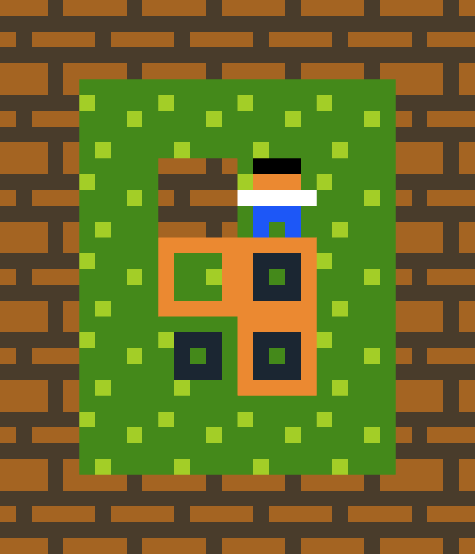
\includegraphics[width=0.5\linewidth]{figures/sokobaniteratelevel.png}
\caption[SokobanIterate]{Sokoban level participants were prompted to iterate upon\label{fig:sokobaniterate}}
\end{figure}

% Interestingly, not all designers we interviewed followed (or even attempted) to use the iterative design method. We believe this might be because these designers either tried to fit their own method onto the tool (with varying degrees of success) or started to play around with the tool to exploit all the possible ways of creating levels.


\subsection{Iterative design}

The iterative design approach was the primary way we intended users to design levels. We encountered this method in our need-finding survey and in blog posts of Sokoban designers \footnote{\url{http://sokoban-jd.blogspot.com/2015/02/how-to-build-sokoban-level.html} @ How to build a Sokoban level -- Serg Belyaev}. The design process roughly looks as follows:

\begin{enumerate}
\item Have a set of rules for the puzzle game.
\item Create an aesthetically pleasing level / decide on a
theme / find an interesting mechanic.
\item Iteratively turn this construction into an enjoyable level.
\end{enumerate}

Most of our participants (2,3,4,5,6,7) have, among others, employed this method while designing their Sokoban level.
A good way of illustrating how users iterated upon their design is to look at how participant 6 used the tool. The corresponding design can be seen here \ref{fig:part6iterative}:

\hspace{\dimexpr-\fboxrule-\fboxsep\relax}\fbox{%
\begin{minipage}{\textwidth}
First, he started by employing the `do a bit of everything' transformation on the presented Sokoban level to go from the initial design to a design with two crates and two targets and one additional crate at the right. He removed this crate and decided that he likes the two crates, two target configuration and planned to design a level around it. When prompted, he said he liked it aesthetically and because it had two interesting solutions. \hfill \\

Next, he decided to remove as much from the top of the level as possible (we think this is because he wanted to disable the solution through the hoop). He continued doing this until he found that the last wall he placed made the level unsolvable (as reported by the mixed-initiative system). As soon as this happened, he then decided to let the transformer make it `somehow work' again (after saving a copy of the design). This was a pattern we frequently saw designers take: As soon as their design became unsolvable, they decided to let the transformer make it somehow work again through transformations. \hfill \\

From there, he picked a few that looked interesting and decided to build on one of them. Because our mixed-initiative system optimized for levels that have a lot of possible states (which are easily identifiable as dead ends to the player), it often generated levels with some unnecessary space. Our participant then finalized the design by removing these unnecessary dead ends. Again, this was a pattern we frequently observed: The transformer (or the designer) made a level which had redundant parts which then had to be manually removed.
\end{minipage}
}

In the next section, we try to list some of these re-occurring design patterns, analyze them, and compare them with the literature. 

% Unfortunately, not all participants had a very smooth experience with the tool. Especially participant 5 immediately decided that impressive Sokoban levels were massive and would contain many crates which unfortunately the transformer did not handle very well. The designer then had to limit himself to designs that the transformer supported.

% Other complaints included user interface issues which are now dealt with in newer versions.




%Participant 1 \& 4 did not use the tool in an interactive fashion but surprisingly found other ways of utilizing the transformation tool (see other sections).

% Interestingly, the game designers we interviewed who did not have much experience with designing puzzle games followed the iterative design the most. We believe this might be because more experienced developers either tried to fit their method onto the tool (with varying degrees of success) or started to play around with the tool to exploit all the possible ways of creating levels.

% Participants 2, 3, 5, 6, 7 have attempted to use this method in their design.


\begin{figure}[!htbp]
\centering
\begin{minipage}[t]{0.2\textwidth}
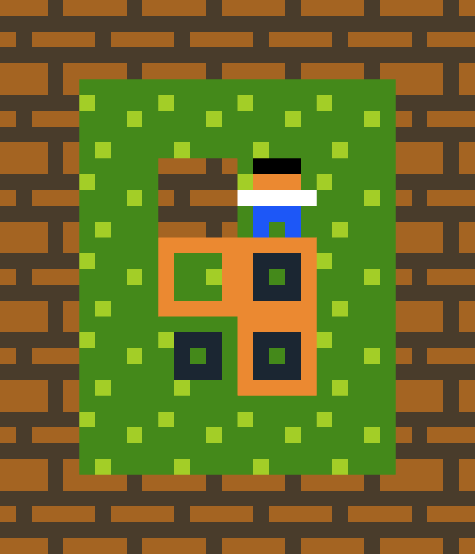
\includegraphics[width=\textwidth]{figures/sokobaniteratelevel.png} \hfill \\
\end{minipage}
$\Longrightarrow$
\begin{minipage}[t]{0.2\textwidth}
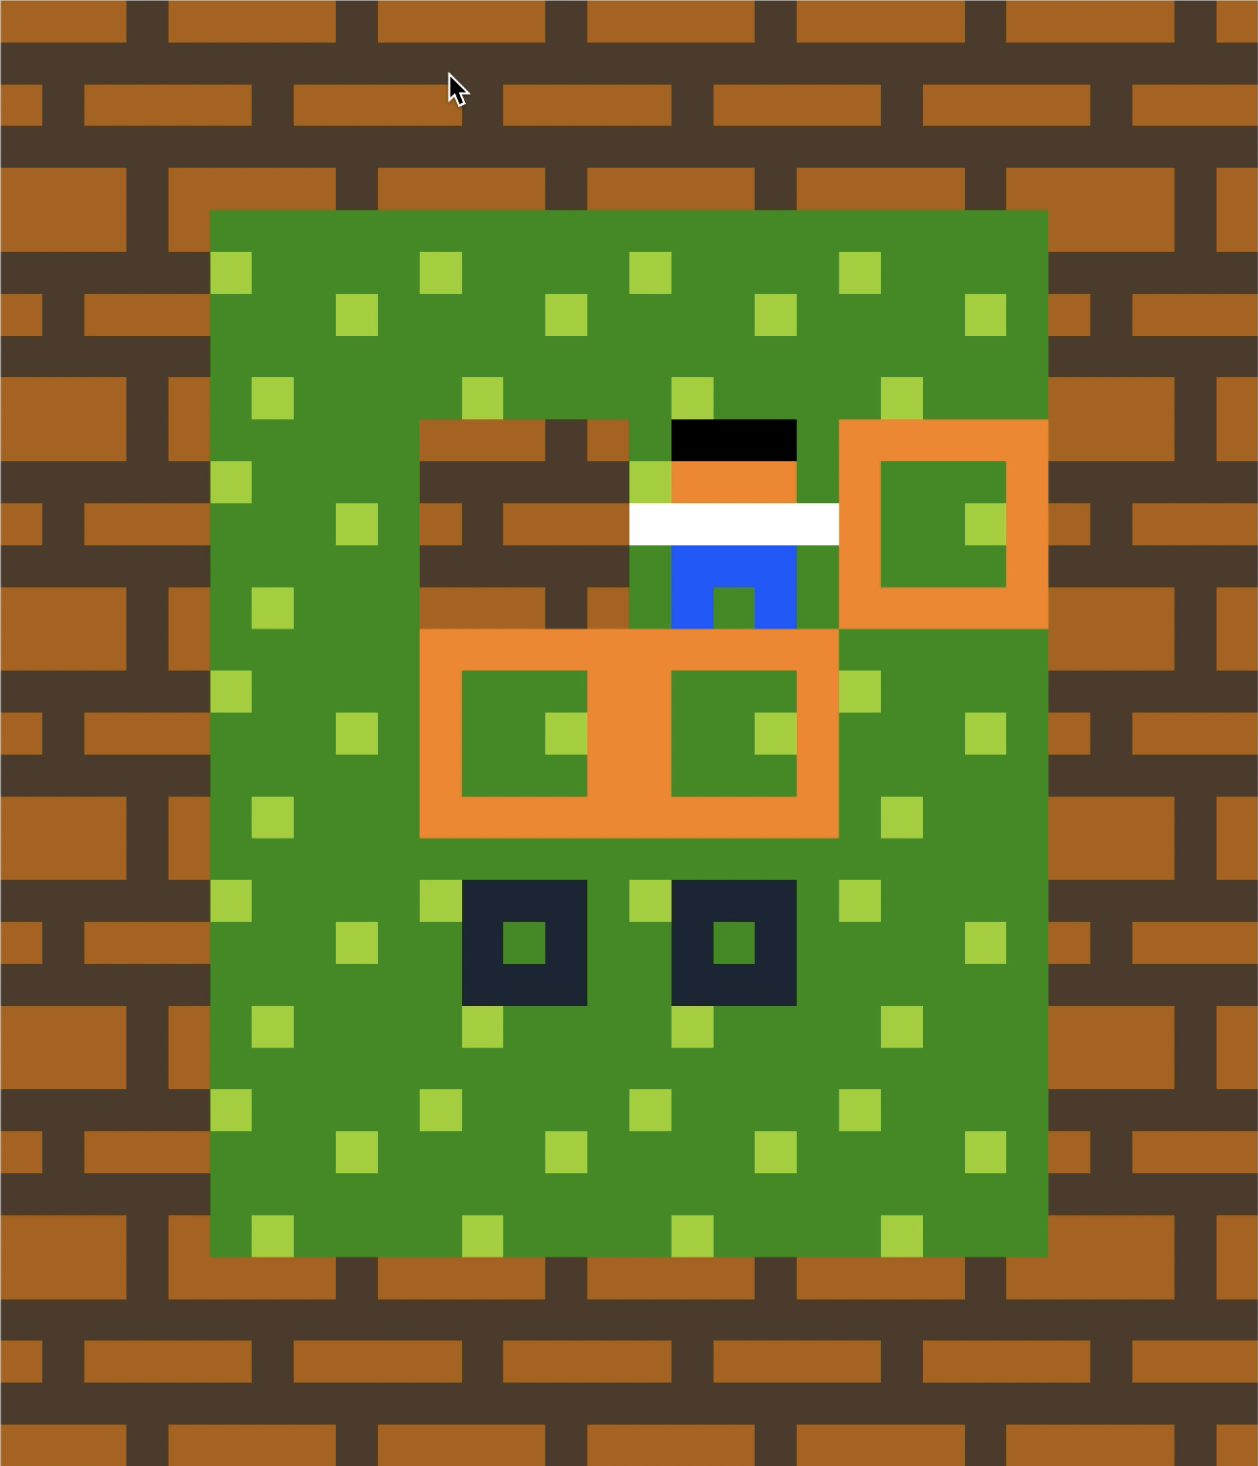
\includegraphics[width=\textwidth]{figures/maxii0.png} \hfill \\
\end{minipage}
$\Longrightarrow$
\begin{minipage}[t]{0.2\textwidth}
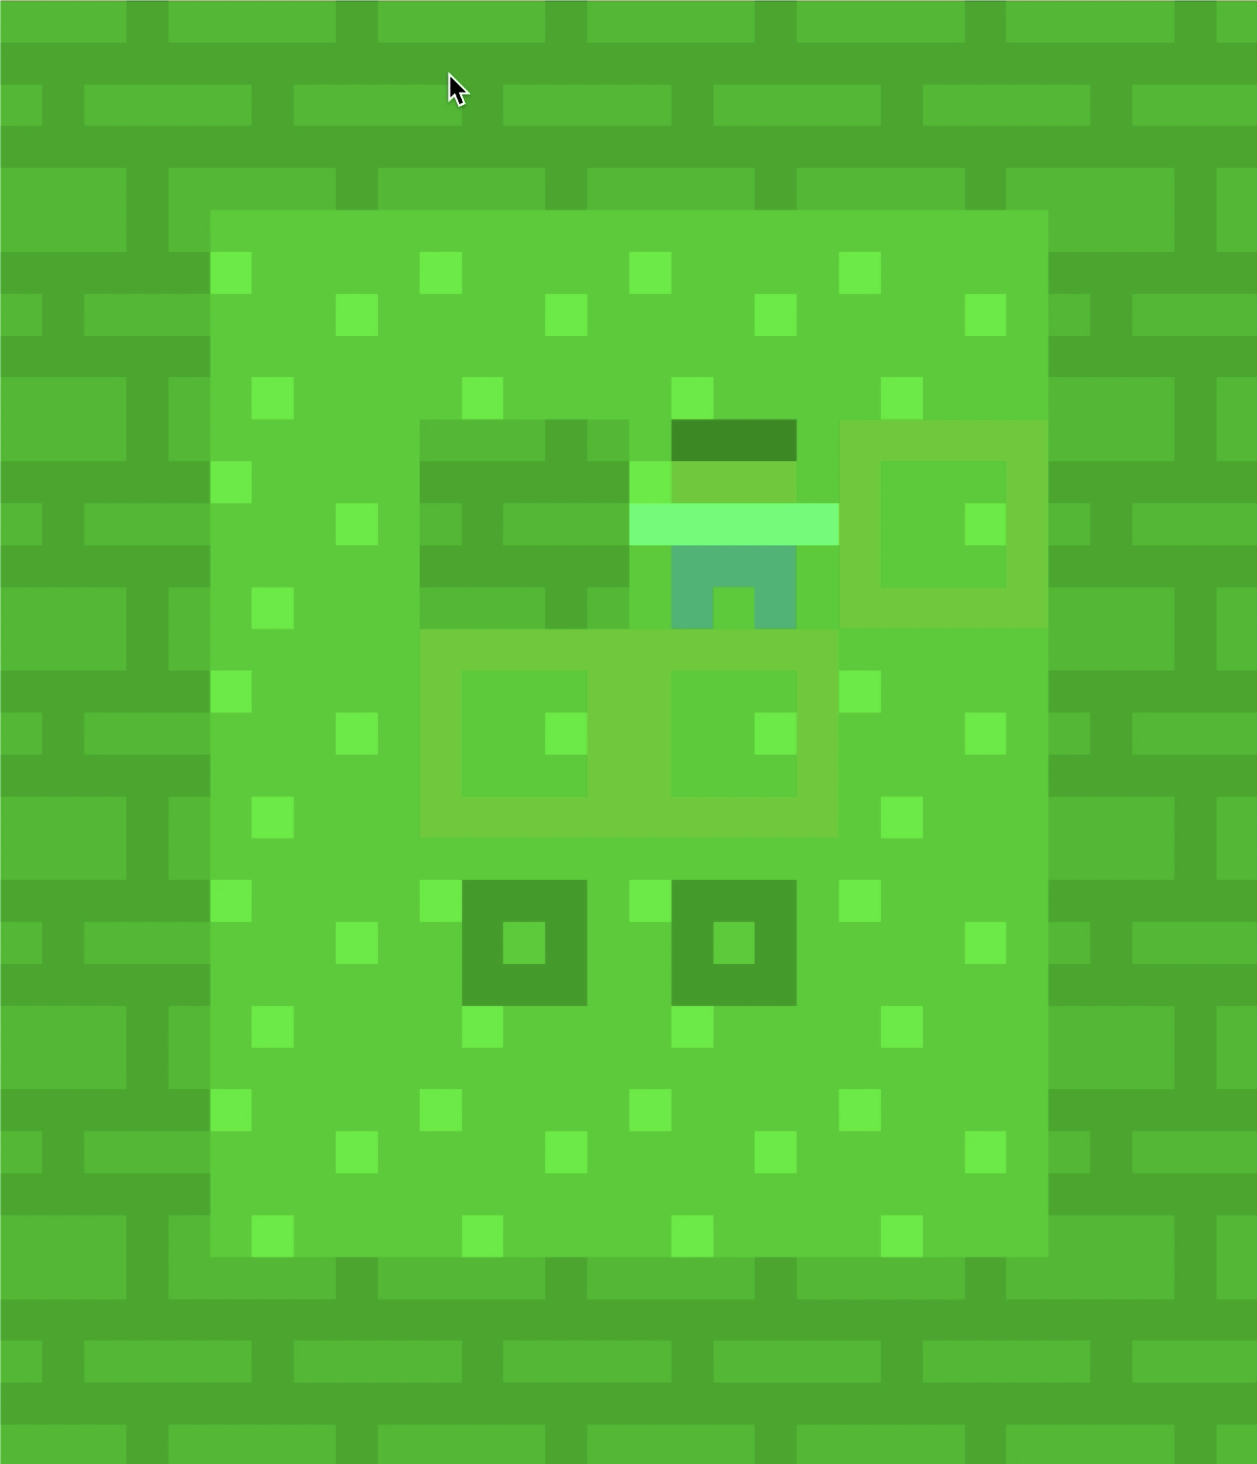
\includegraphics[width=\textwidth]{figures/maxii1_green.png} \hfill \\
\end{minipage}
$\Longrightarrow$
\begin{minipage}[t]{0.2\textwidth}
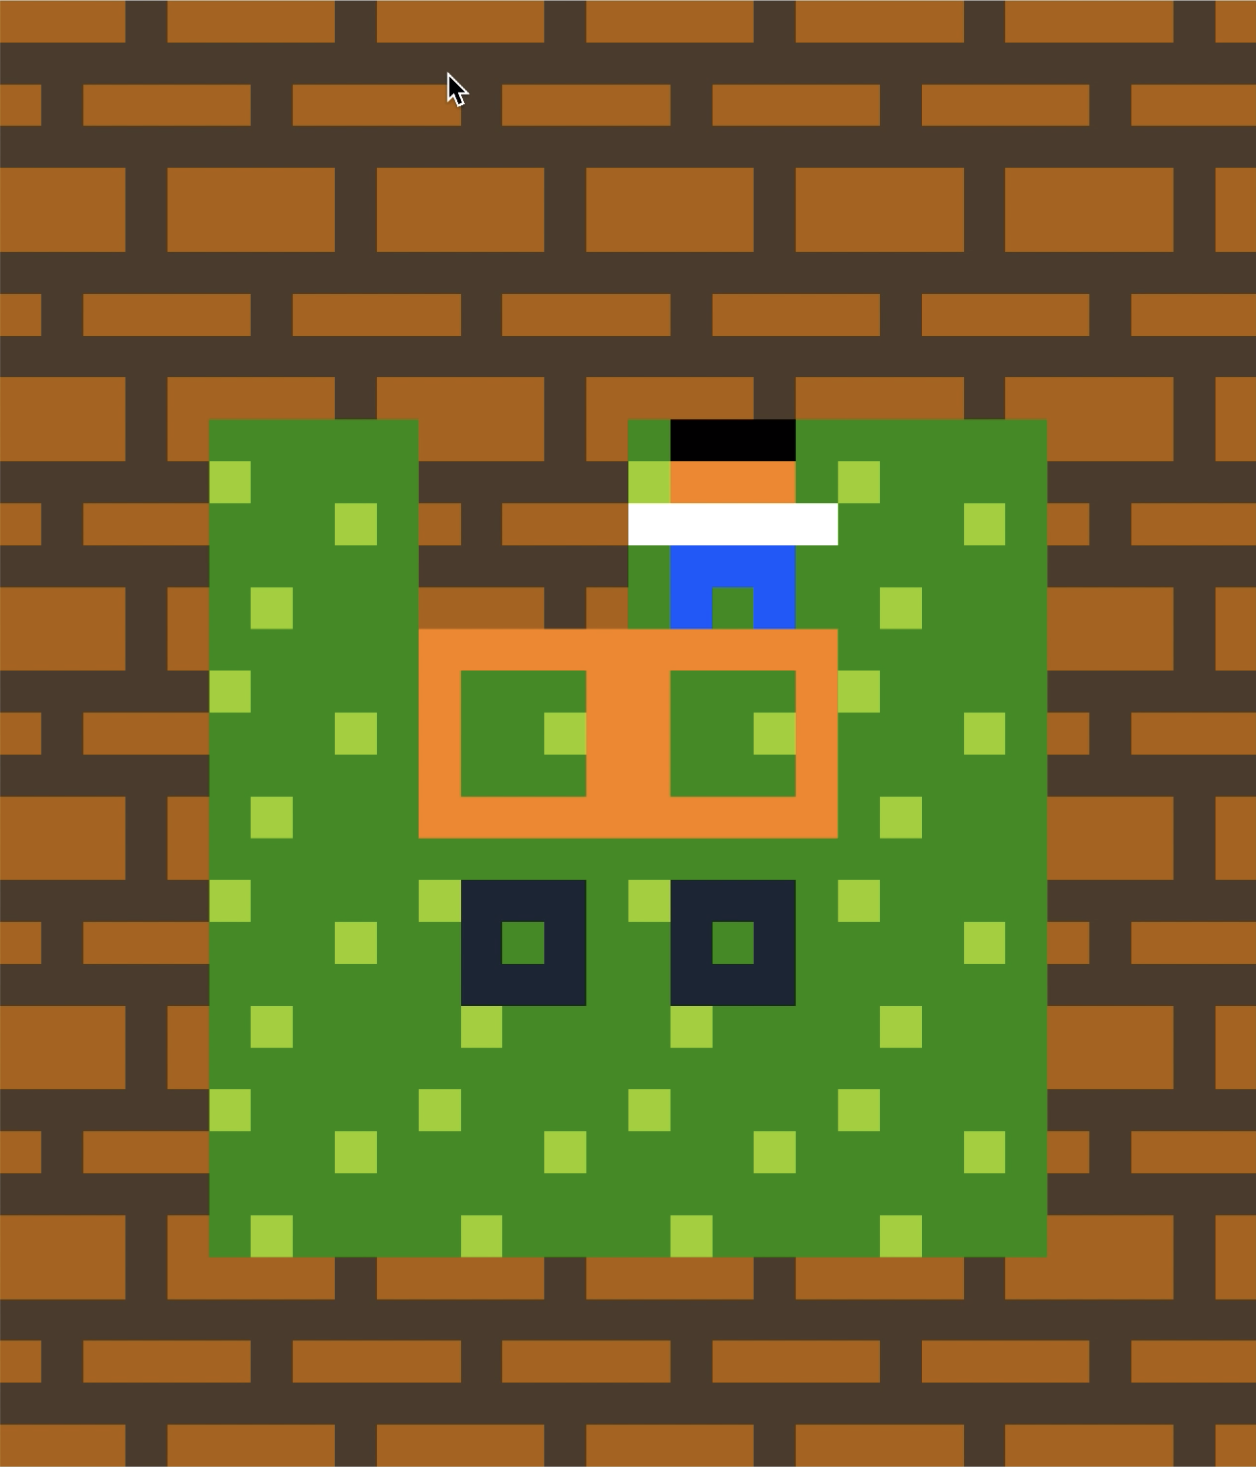
\includegraphics[width=\textwidth]{figures/maxii2.png} \hfill \\
\end{minipage}
$\Longrightarrow$
\begin{minipage}[t]{0.2\textwidth}
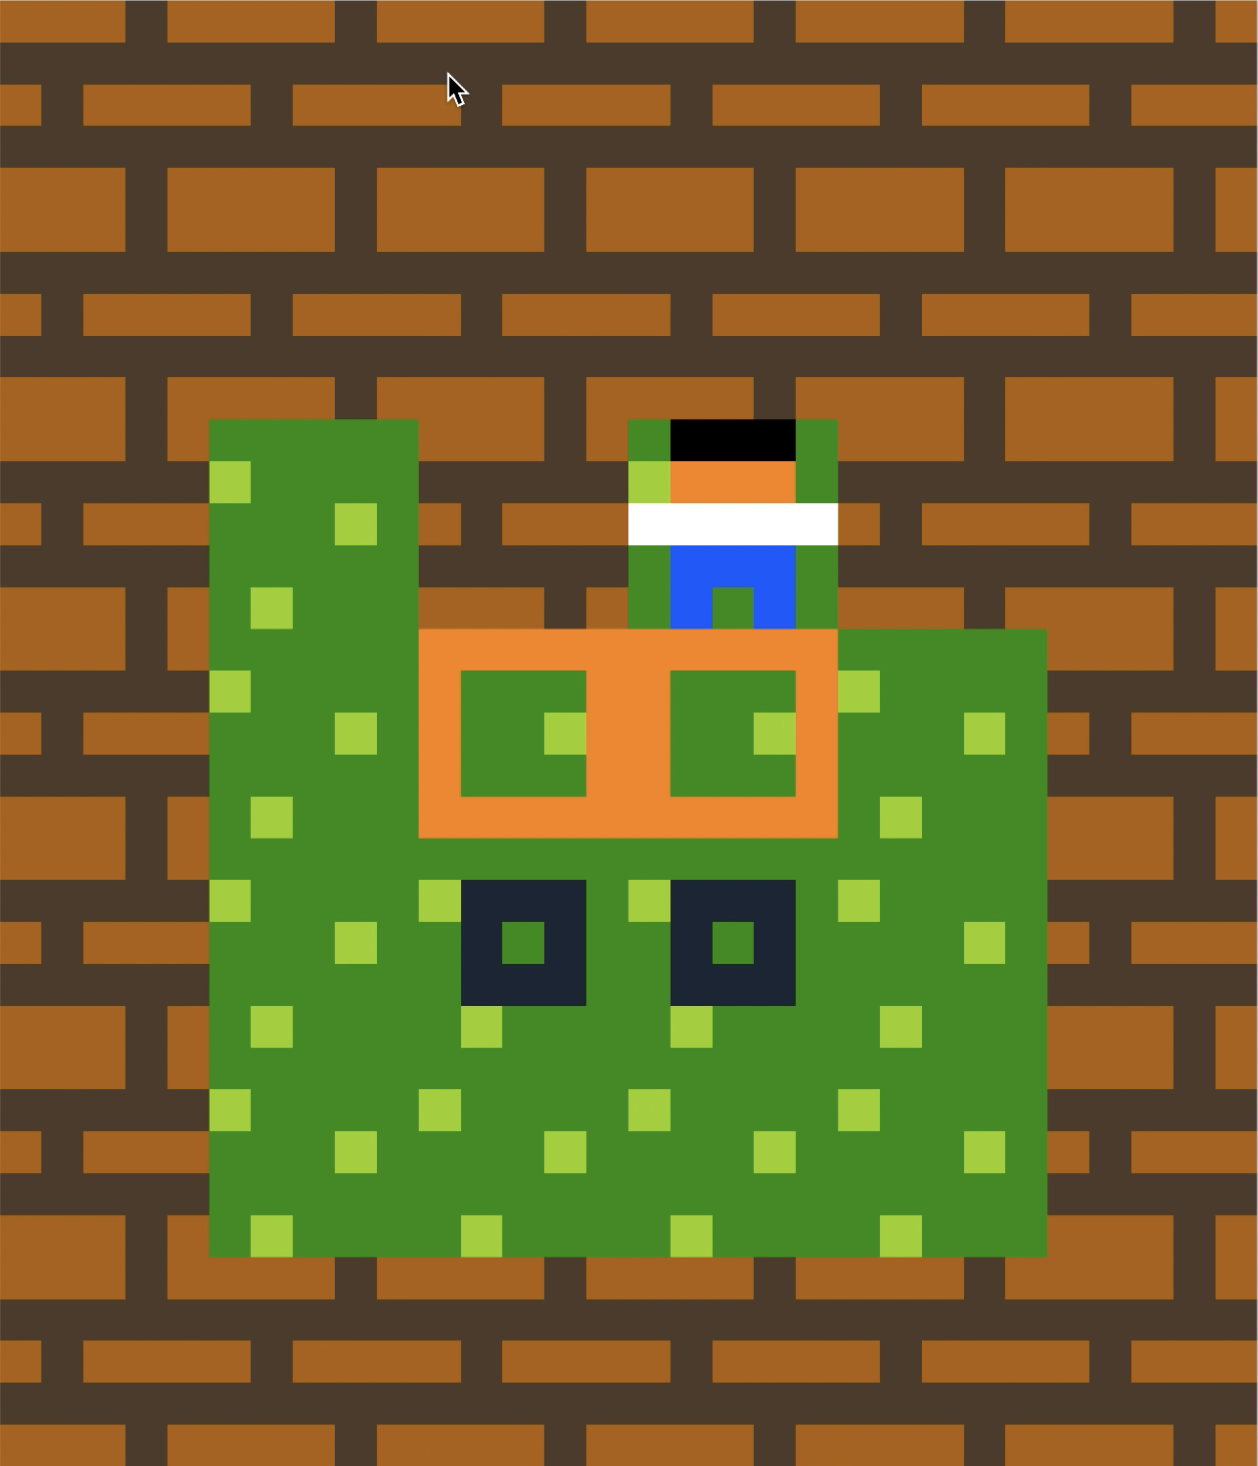
\includegraphics[width=\textwidth]{figures/maxii3.png} \hfill \\
\end{minipage}
$\Longrightarrow$
\begin{minipage}[t]{0.2\textwidth}
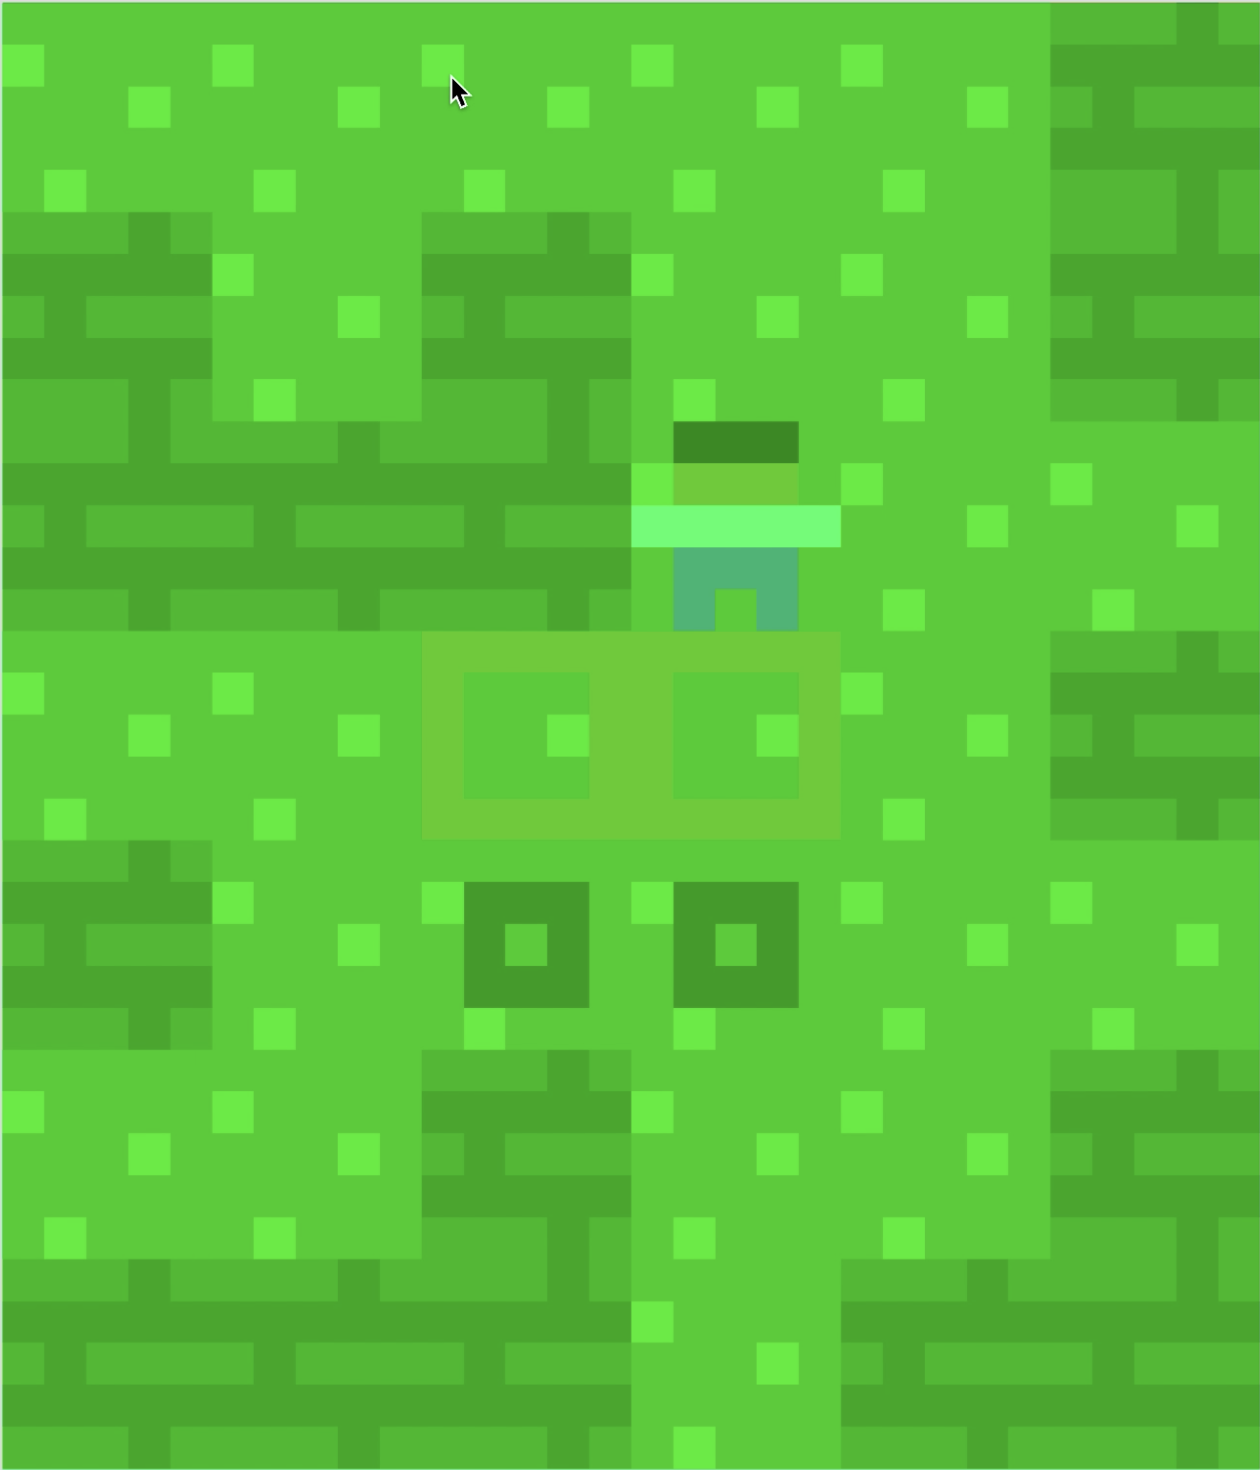
\includegraphics[width=\textwidth]{figures/maxii4_green.png} \hfill \\
\end{minipage}
$\Longrightarrow$
\begin{minipage}[t]{0.2\textwidth}
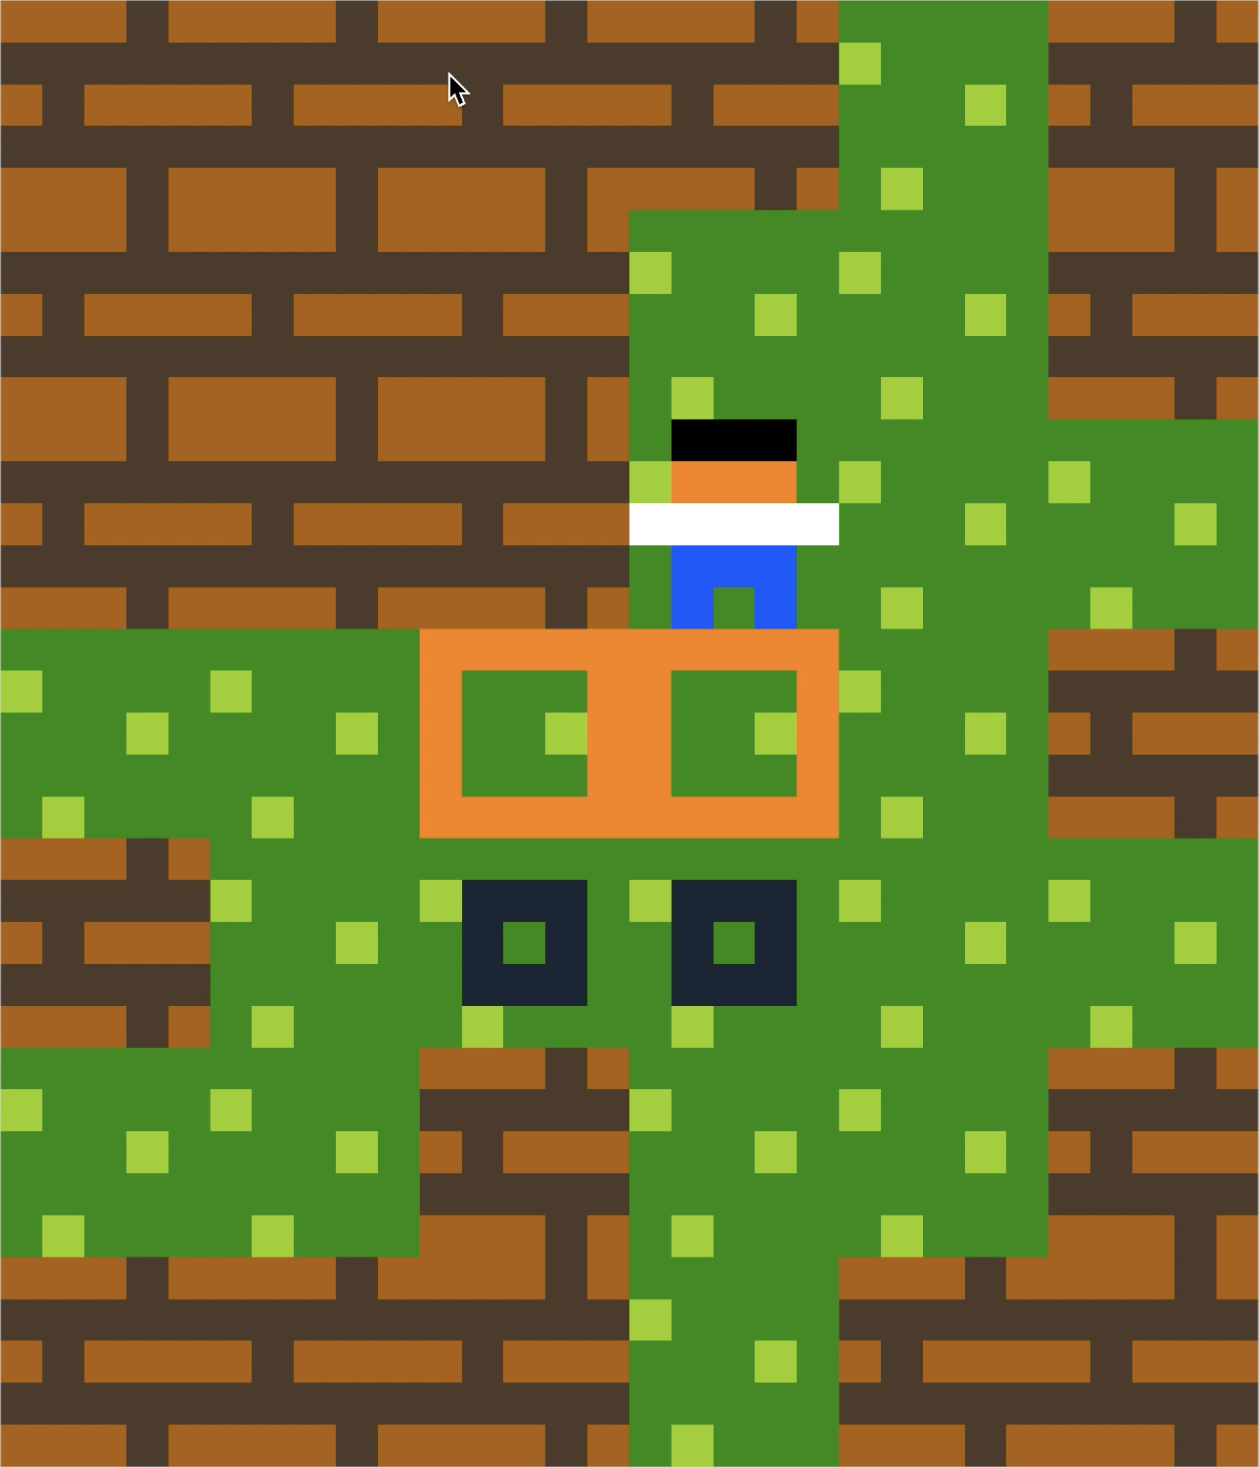
\includegraphics[width=\textwidth]{figures/maxii5.png} \hfill \\
\end{minipage}
$\Longrightarrow$
\begin{minipage}[t]{0.2\textwidth}
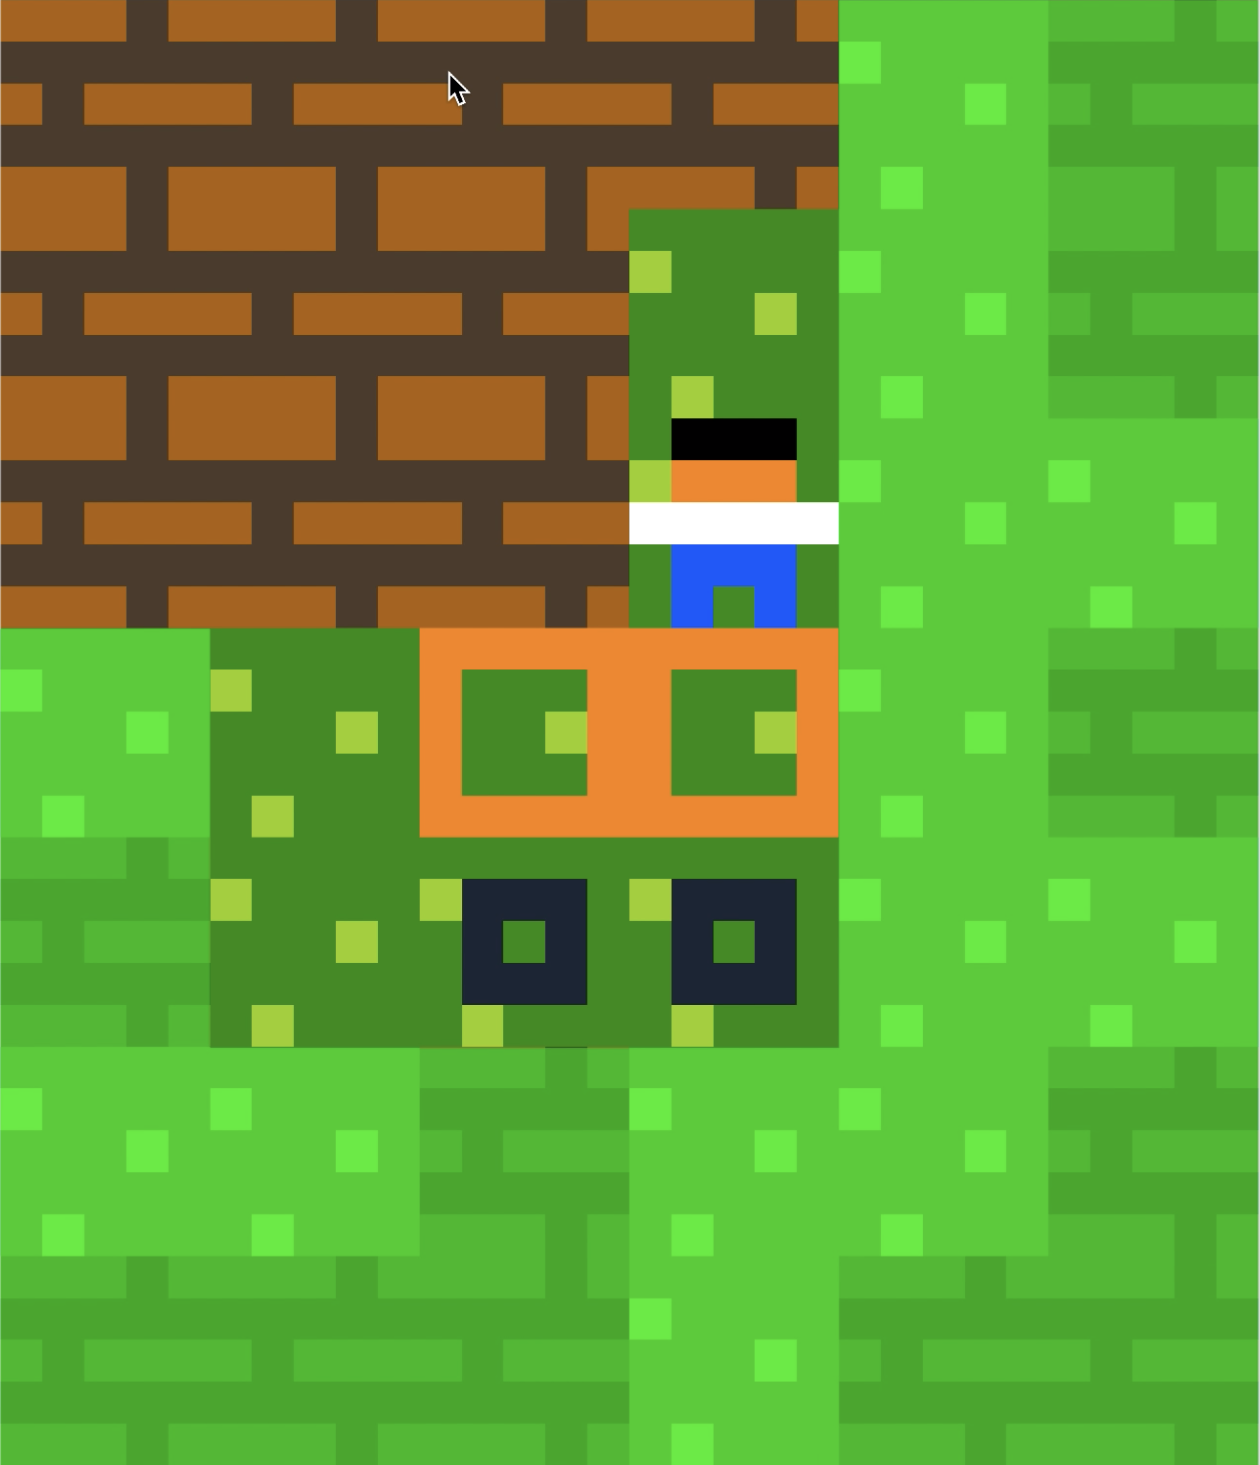
\includegraphics[width=\textwidth]{figures/maxii6.png} \hfill \\
\end{minipage}
$\Longrightarrow$
\begin{minipage}[t]{0.2\textwidth}
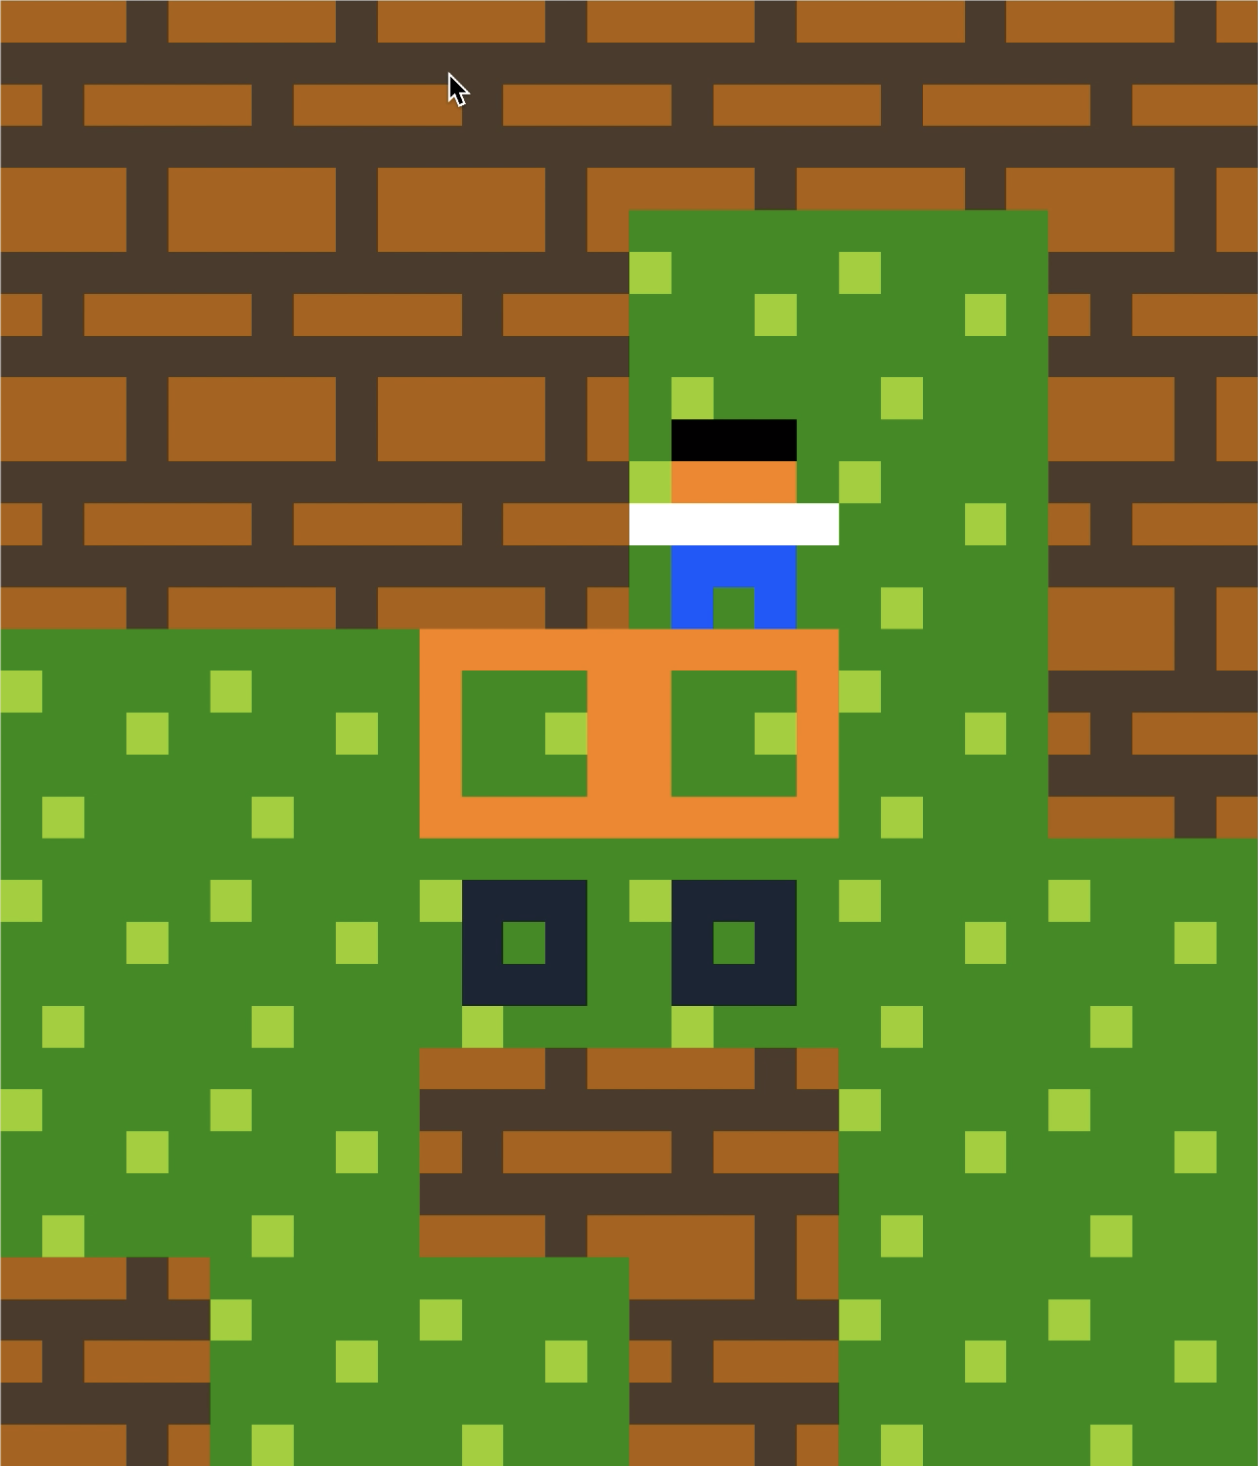
\includegraphics[width=\textwidth]{figures/maxii7.png} \hfill \\
\end{minipage}
$\Longrightarrow$
\begin{minipage}[t]{0.2\textwidth}
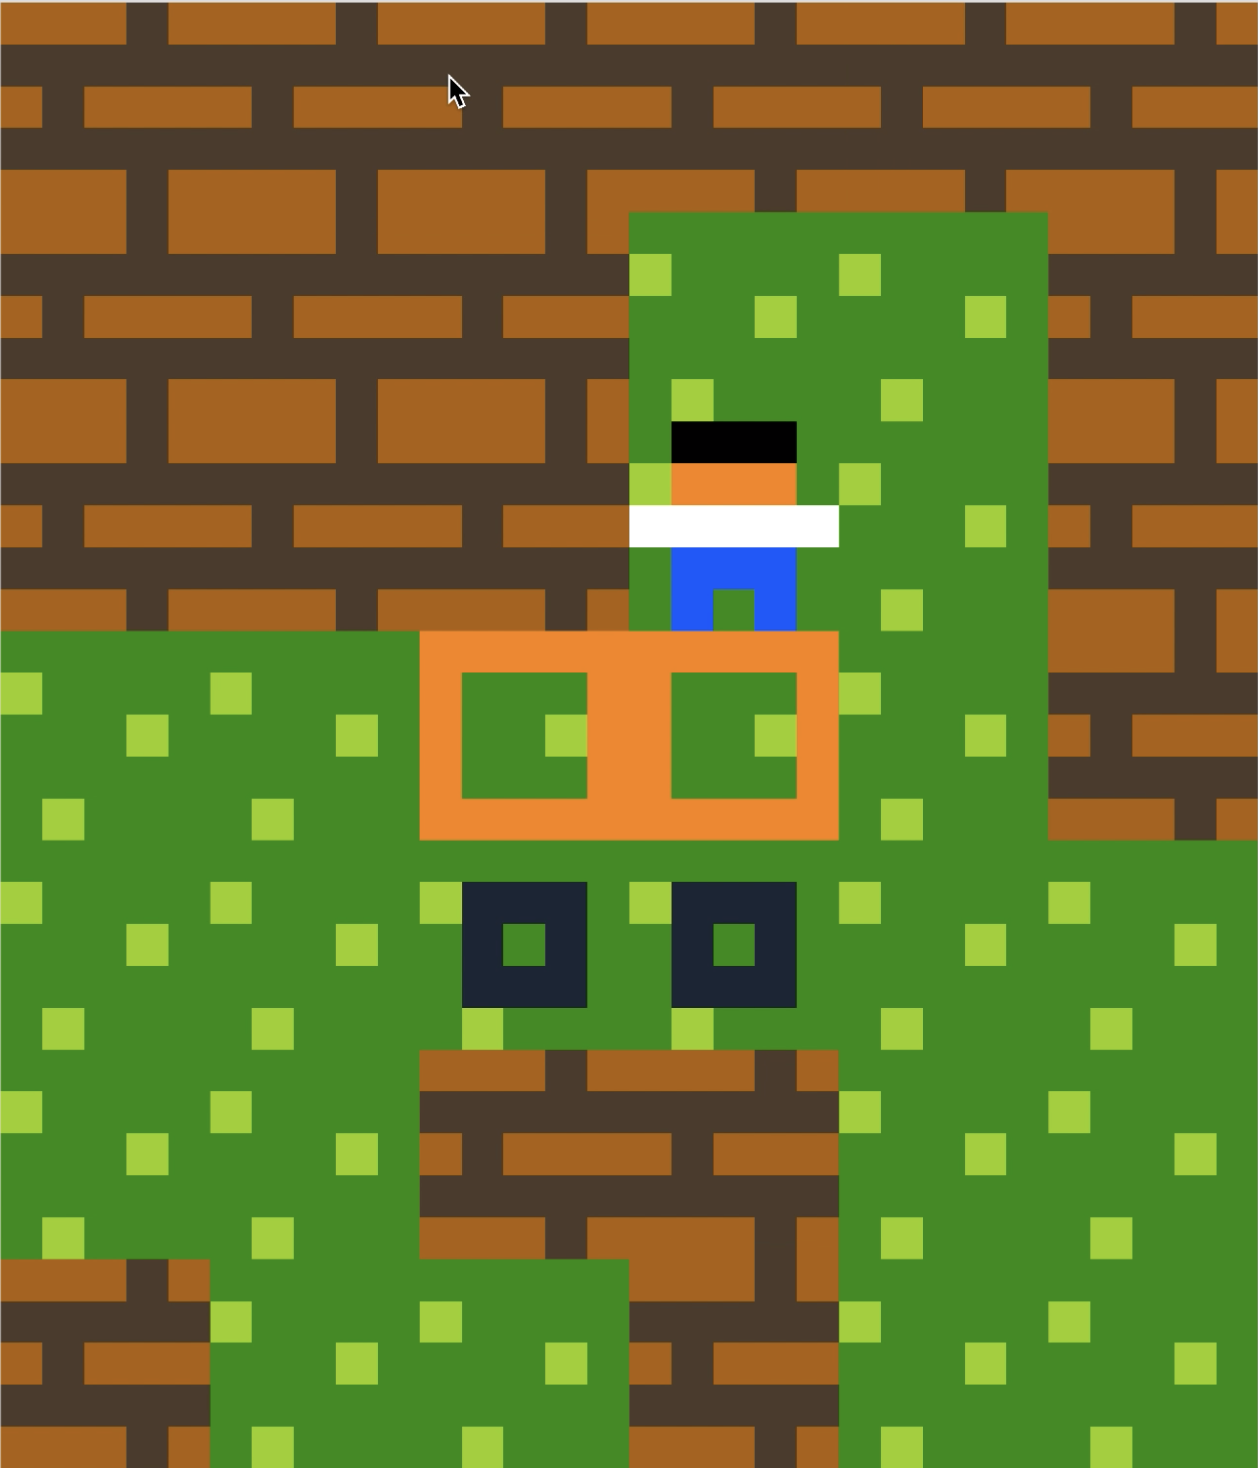
\includegraphics[width=\textwidth]{figures/maxii8.png} \hfill \\
\end{minipage}
\caption{Participant 6: Iterative design processed \label{fig:part6iterative}}
\end{figure}



\begin{figure}[!htbp]
\begin{minipage}{0.5\textwidth}
\centering
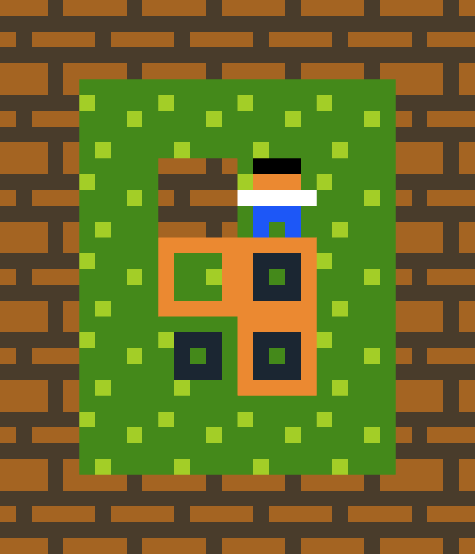
\includegraphics[width=0.55\textwidth]{figures/sokobaniteratelevel.png}

\end{minipage}  $\Longrightarrow$ \hfill
\begin{minipage}{0.4\textwidth}
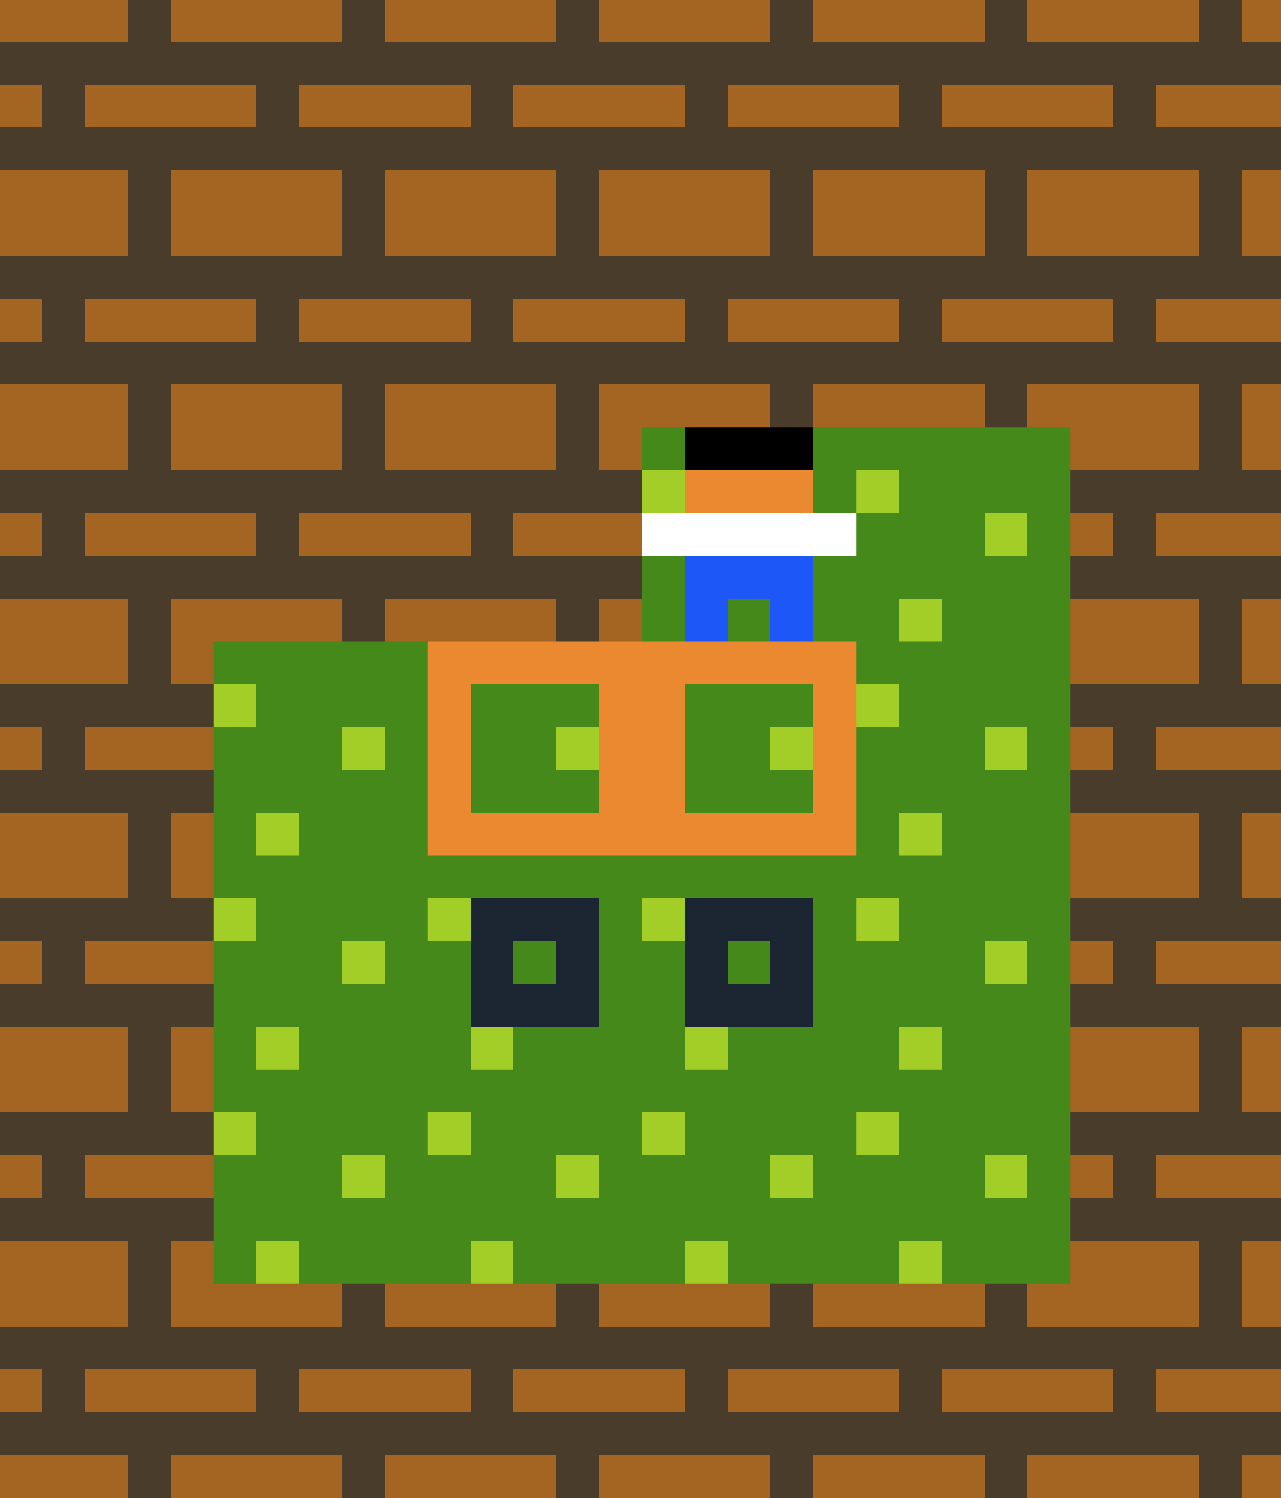
\includegraphics[width=0.55\textwidth]{figures/firstmax_without.png} \hfill \\
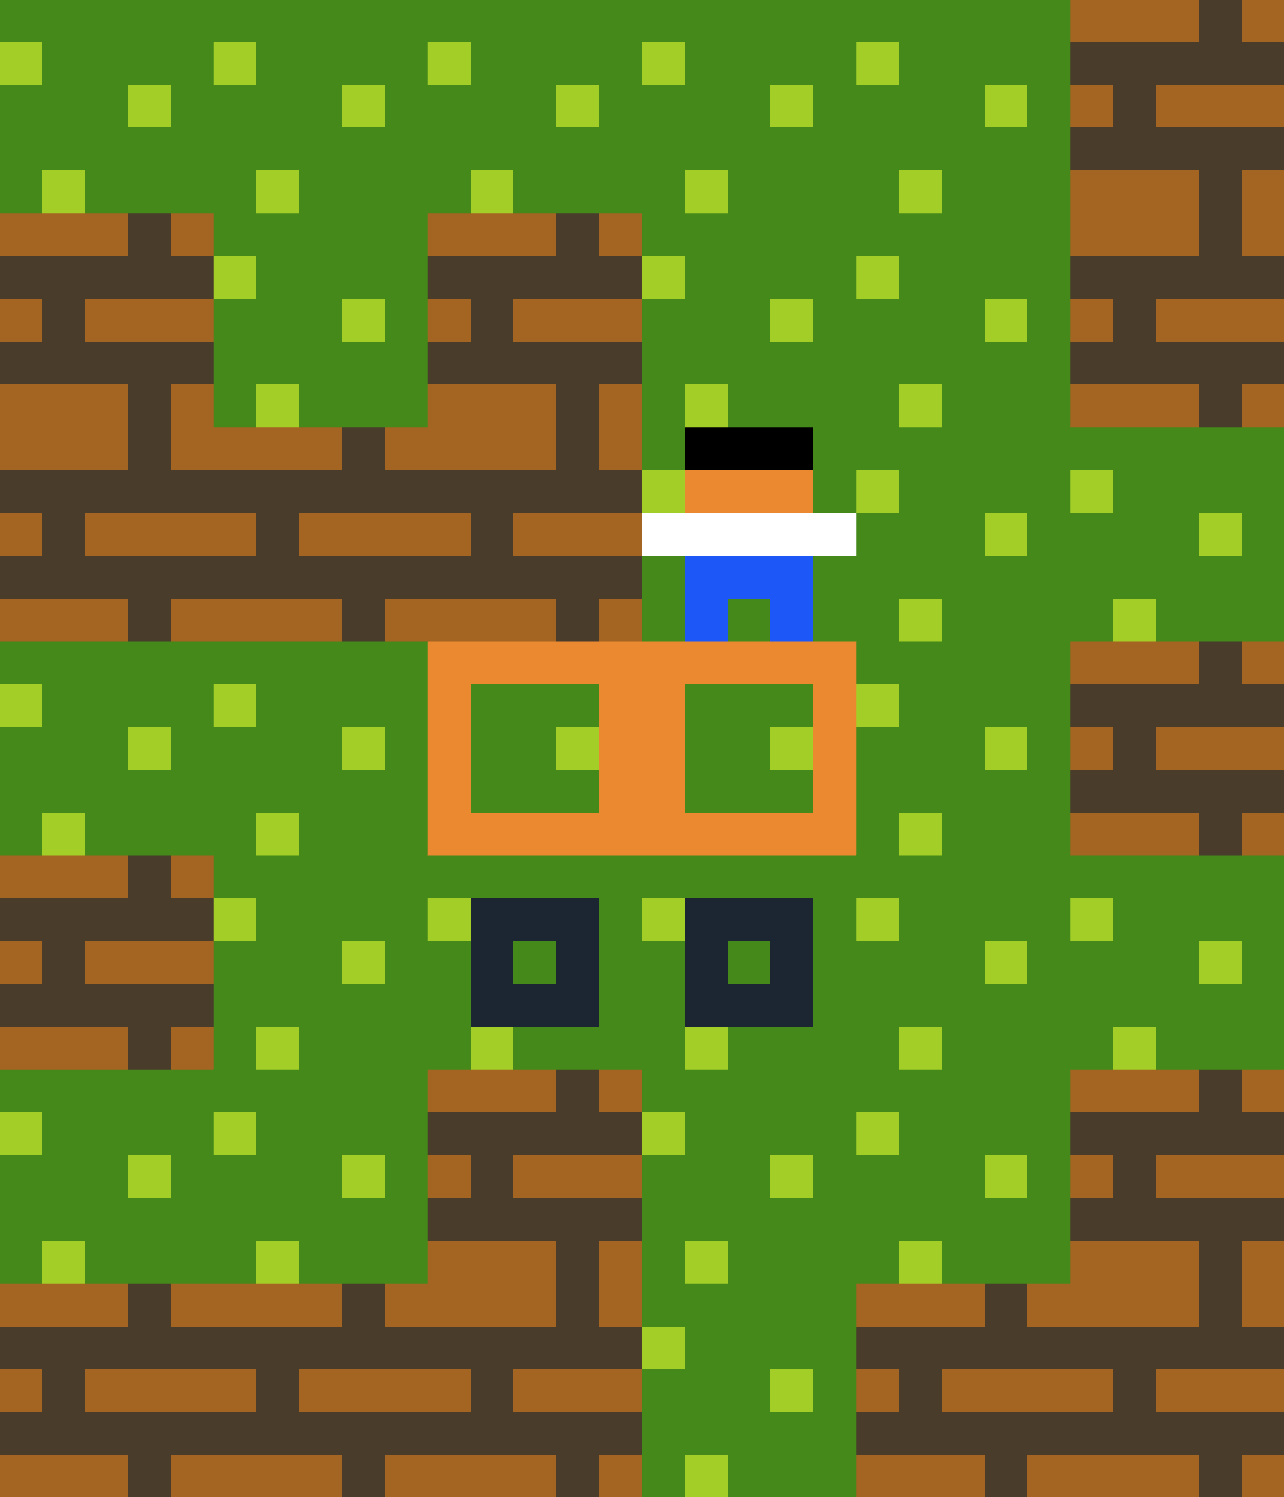
\includegraphics[width=0.55\textwidth]{figures/secondmax_without.png} \hfill \\
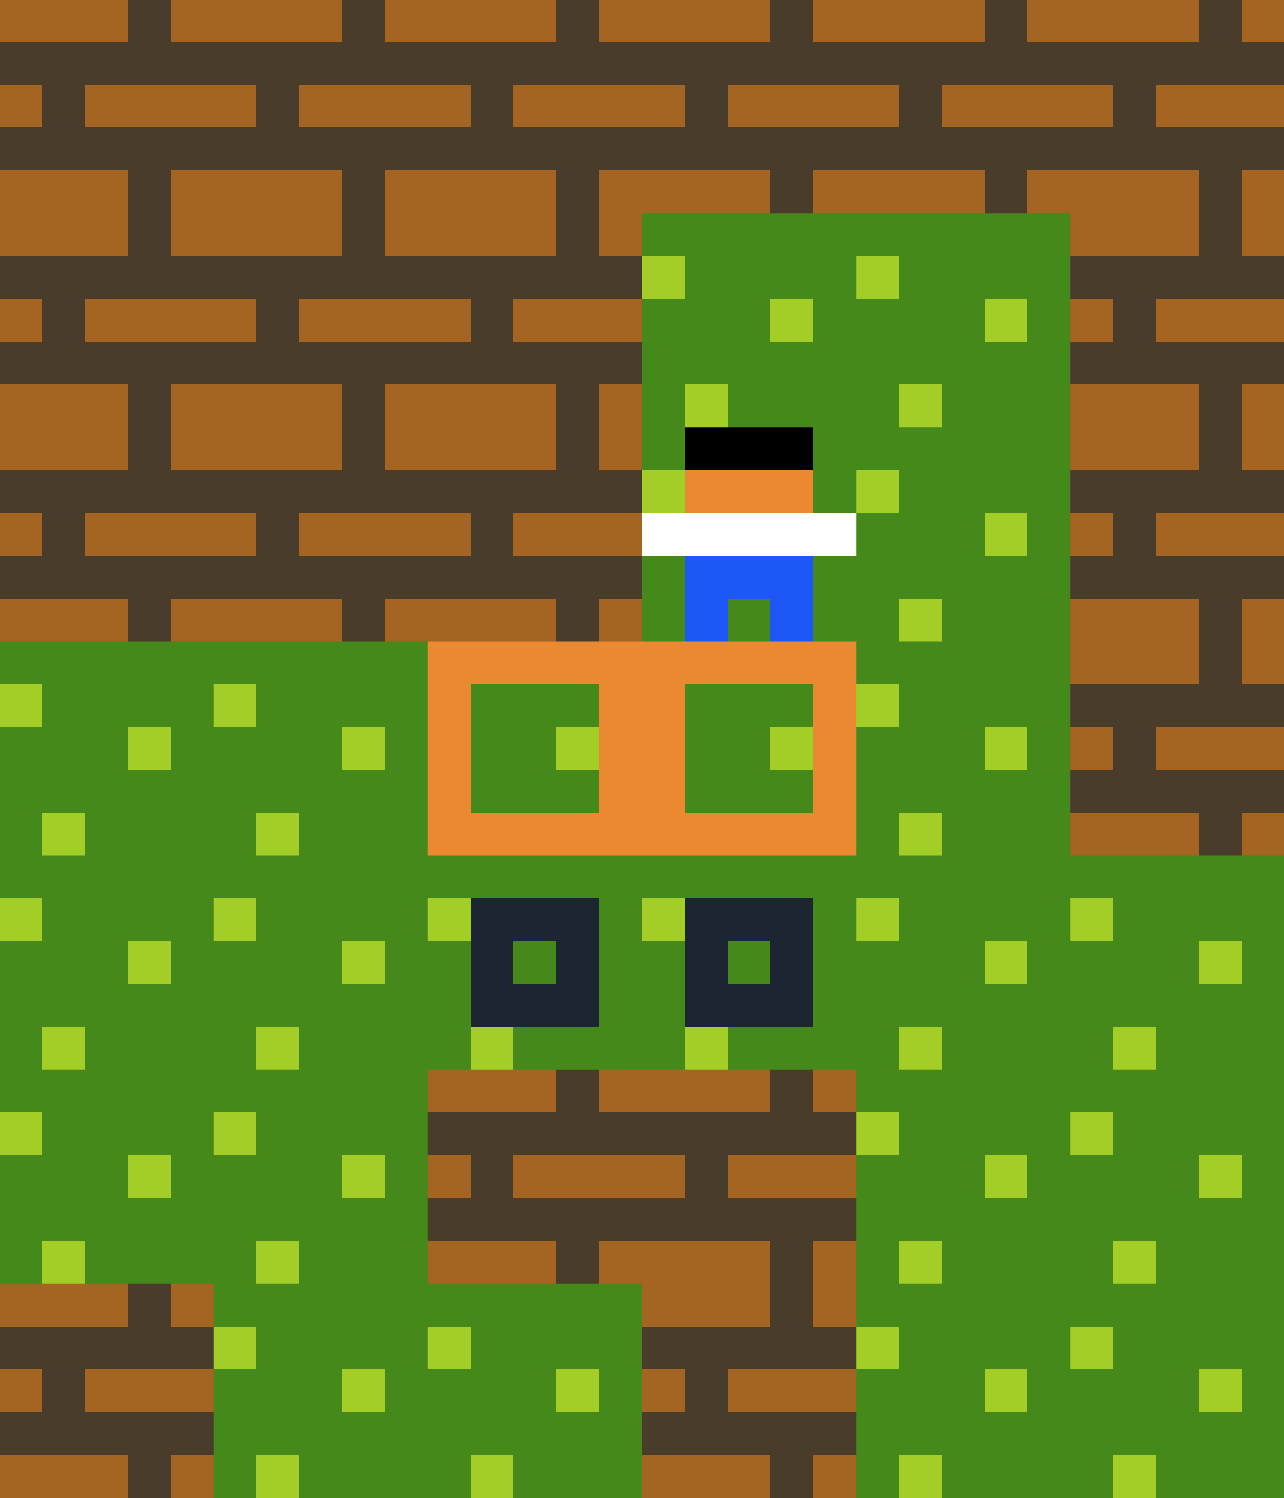
\includegraphics[width=0.55\textwidth]{figures/thirdmax_without.png} \hfill \\
\end{minipage}
\caption{Participant 6: Final iterative designs}
\end{figure}


\begin{figure}[!htbp]
\centering
\begin{minipage}[t]{0.2\textwidth}
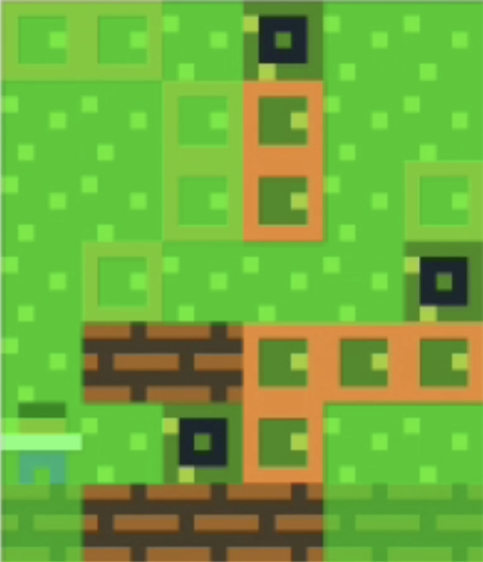
\includegraphics[width=\textwidth]{figures/p8greena.png} \hfill \\
\end{minipage}
$\Longrightarrow$
\begin{minipage}[t]{0.2\textwidth}
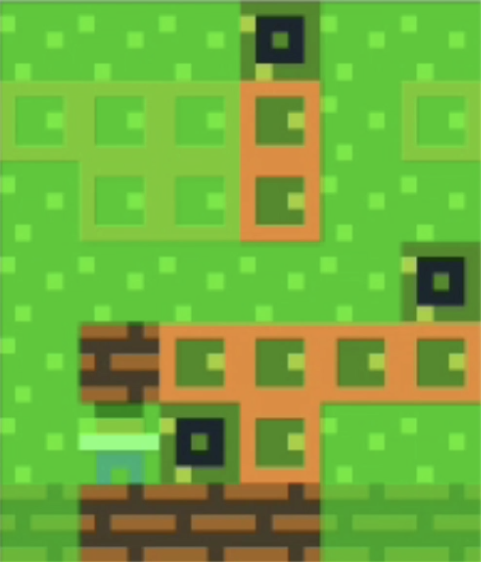
\includegraphics[width=\textwidth]{figures/p8greenb.png} \hfill \\
\end{minipage}
$\Longrightarrow$
\begin{minipage}[t]{0.2\textwidth}
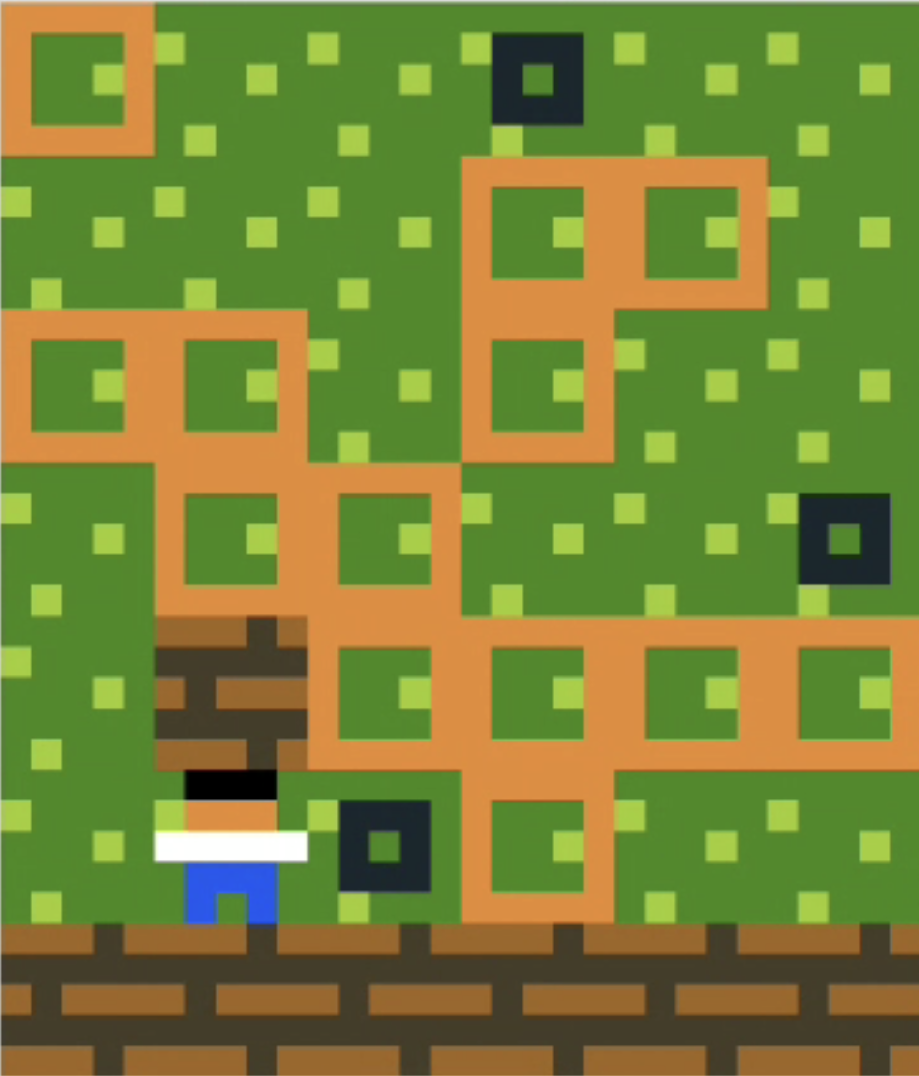
\includegraphics[width=\textwidth]{figures/p8greenc.png} \hfill \\
\end{minipage}

\caption{Participant 7: Iterative design process}
\end{figure}


\subsection{Design patterns}

In this section, we list design patterns for the iterative design approach which we obtained from the think-aloud study and see in which way participants profit from mixed-initiative methods.


\begin{description}
\item[Identifying aesthetics/mechanics] After using the tool for a while, many our participants have found \textit{aesthetically} pleasing sections or \textit{mechanically} interesting sections upon which they liked to expand on. For example, participant 6 liked the two targets and crates in the design mentioned above.

%Especially participant 1, 2 \& 4 have used the tool mostly for this purpose considerable time with the other aspect of the mixed-initiative tool: Finding it for inspiration.

% They then continue to expand on it with creative constraints, window dress the solution or try to transform a given design using the generator.

MixedAim helped the designer identify some interesting designs by passively suggesting levels during the design phase (5 participants claimed they got inspired by a level without clicking on it) or by the designer explicitly looking for them with the transformer. Especially participants 1, 2 \& 4 focused on using the transformer to come up with original designs upon which they then were able to improve, see also the section 5.1.3. 

\item[Creative constraints] These are situations where designers constrain themselves only to the use of a previously identified aesthetic or mechanic. Every participant worked with creative constraints in one way or the other.

Mixed-initiative tools helped the designer to satisfy \textit{aesthetic constraints} by allowing them to \textit{freeze} certain sections that the transformer would not be able to change. For example, participant 6 decided he would keep the two crates and the two walls and constrained the transformer to only change the level around the crate target pairs. Further suggestions for \textit{aesthetic constraints} followed from the structured interview included adding tools for \textit{symmetry} and being able to \textit{combine} two levels in interesting ways.

For \textit{mechanical constraints}, the transformer rules have to be employed to create interesting mechanics. These are for example the preset buttons like only moving the crates or removing/adding some walls and keeping the rest intact. Suggestions included not only \textit{specifying} ways of transforming but also specifying means of constraining allowed transformations. 

\item[Unsolvable into solvable] This was not something we encountered in the literature, but it was something that happened very frequently with our mixed-initiative system. As soon as designers were passively shown that the level was unsolvable, they did not spend the effort to make it solvable manually but told the tool to make the current design work somehow. A lot of these designers then reported being pleased by the methods the transformer came up with to make the level solvable again.

This was also mentioned directly by participant 3 during the think-aloud study: \textit{\say{A perfect way to use this [tool] is if you find something that looks interesting, but you cannot quite get it to be solvable or something like that.}}

\begin{figure}[!htbp]
\begin{minipage}{0.5\textwidth}
\centering
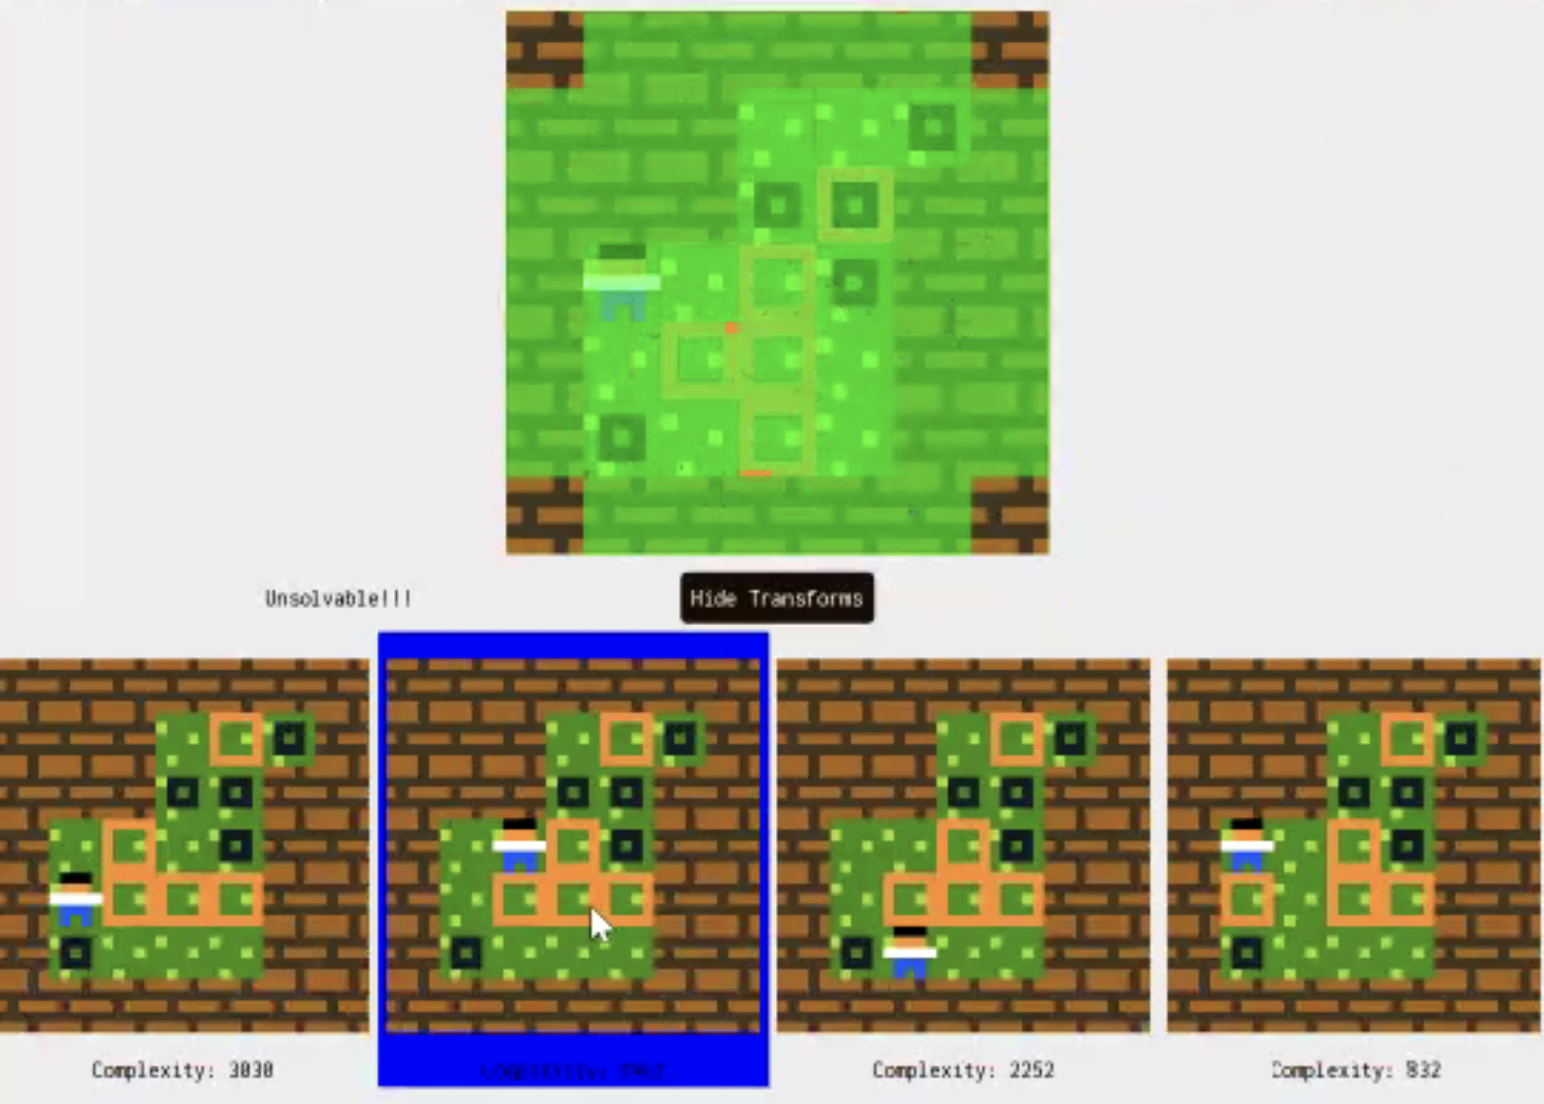
\includegraphics[width=\textwidth]{figures/unsolvablepart4.png}
\end{minipage}  \hfill
\begin{minipage}{0.5\textwidth}
\centering
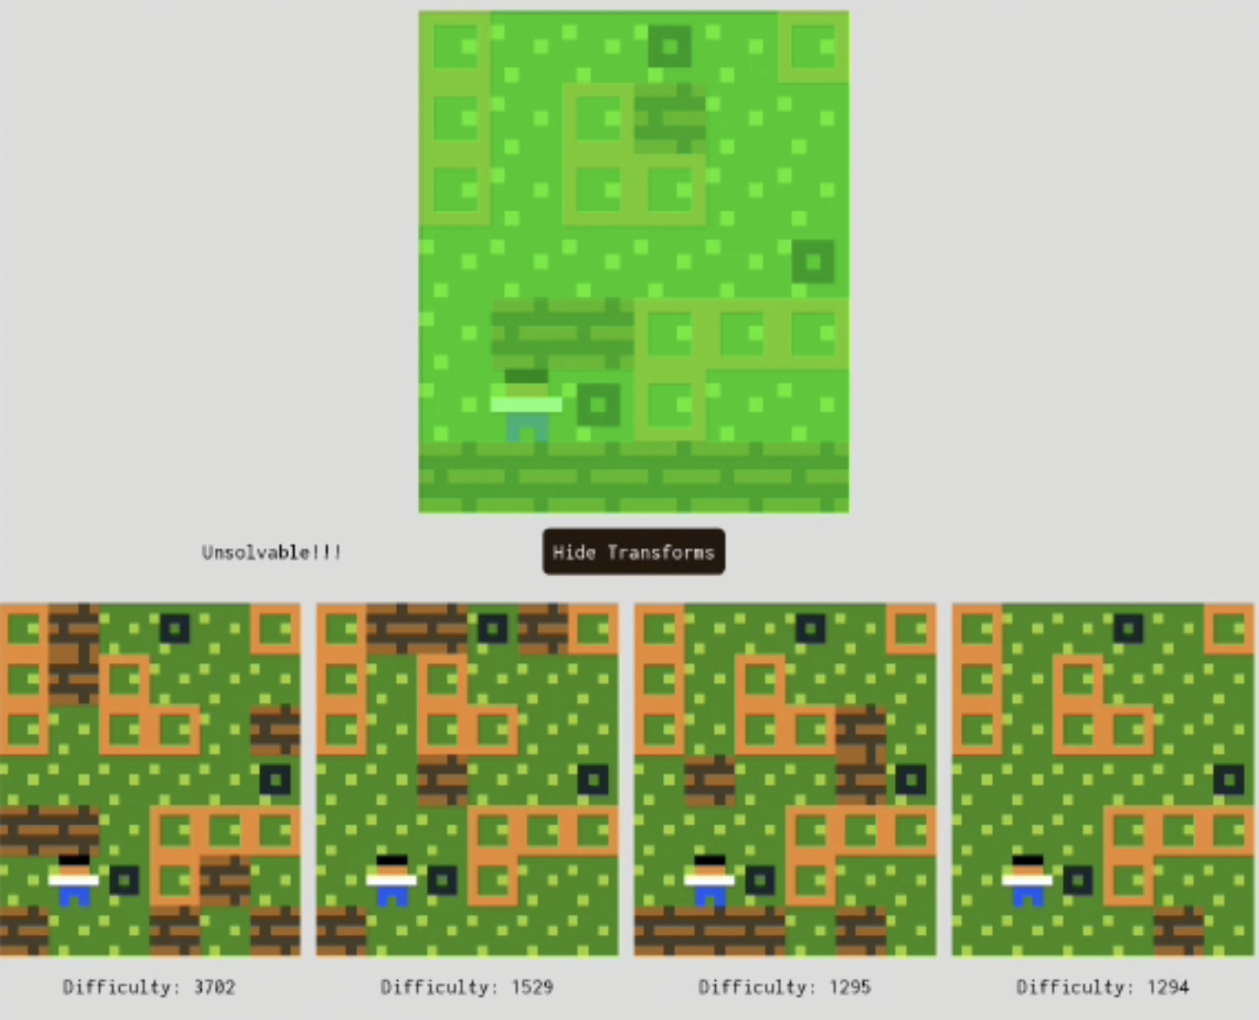
\includegraphics[width=\textwidth]{figures/unsolvablepart72.png}
\end{minipage}
\caption{Participant 4 \& 7: Unsolvable to solvable}
\end{figure}

\item[Window dressing] This happens when an interesting level is found (through the transformer or the designer) that contains a lot of unnecessary states. The designer then tries to eliminate all these unnecessary states (without making the problem trivial) to find the `canonical form', the `kernel' of the problem. It was mentioned by participant 1, 6 \& 7.
%definitely mentioned by participant 1, participant 6, thatscar, and participant 7.

Our mixed-initiative tools only help to address this problem in so far that they help the designer to edit the level quickly. Passive information about solvability can tell the designer whether or not his simplifications suddenly made the level easier, for example. Participant 7 added a figure.

\begin{figure}[!htbp]
\centering
\begin{minipage}[t]{0.25\textwidth}
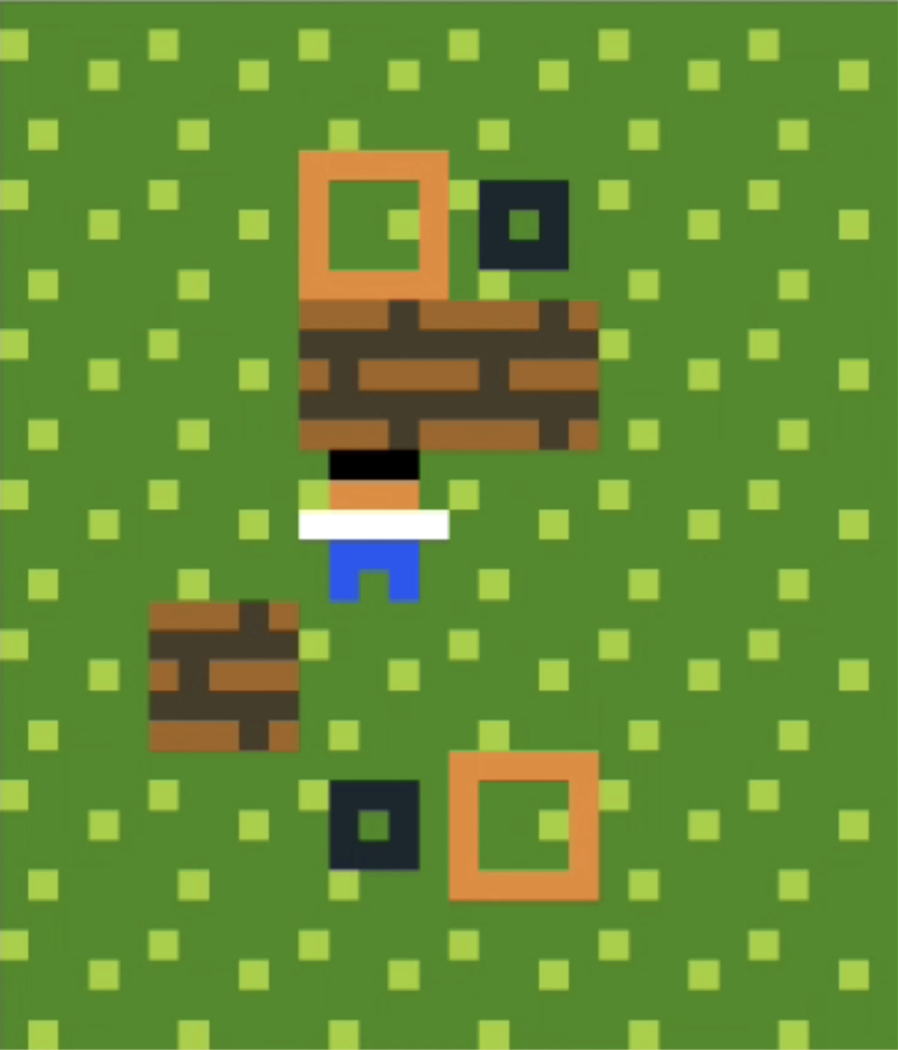
\includegraphics[width=\textwidth]{figures/windowdressingpart71.png} \hfill \\
\end{minipage}
$\Longrightarrow$
\begin{minipage}[t]{0.25\textwidth}
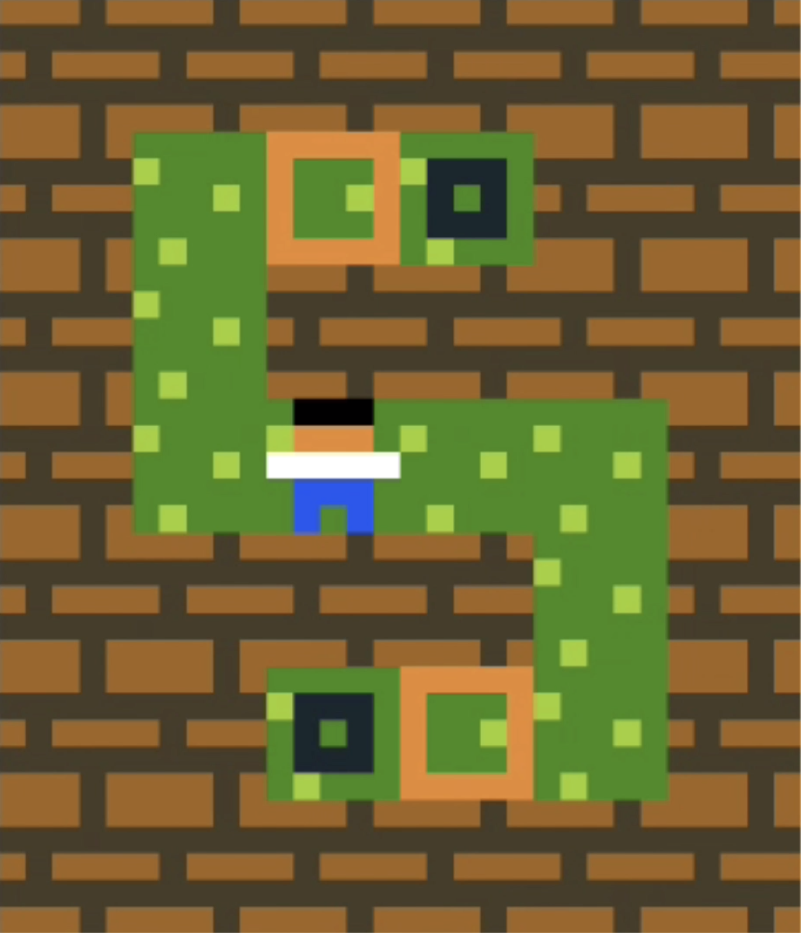
\includegraphics[width=\textwidth]{figures/windowdressingpart72.png} \hfill \\
\end{minipage}
$\Longrightarrow$
\begin{minipage}[t]{0.25\textwidth}
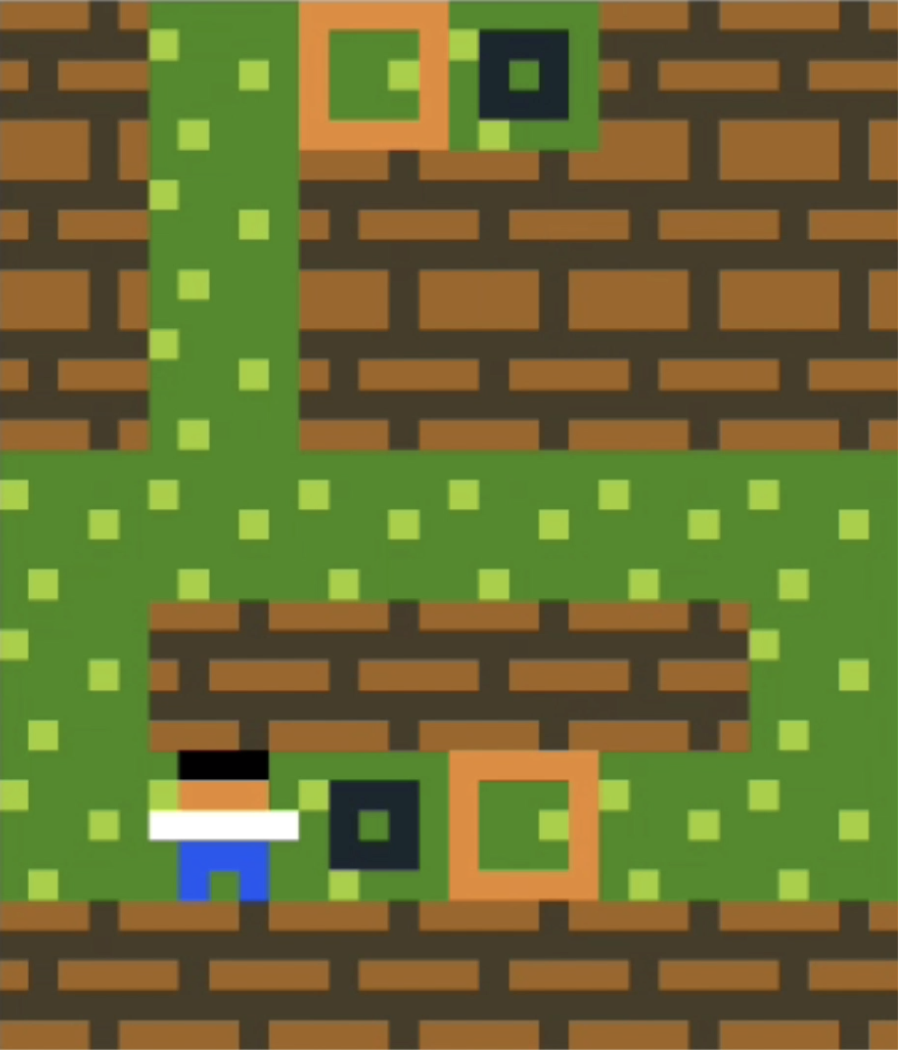
\includegraphics[width=\textwidth]{figures/windowdressingpart73.png} \hfill \\
\end{minipage}
\caption{Participant 7: Window dressing}
\end{figure}
    

\item[Mechanic swapping] Participant 1 already had an extensive library of Sokoban-like PuzzleScript games and used this to utilize the tool in an interesting manner. He loaded up a list of Sokoban levels into the tool and then started to change the rules of the Sokoban game. For example, he made it so players can push the block vertically but only teleport through the block horizontally. After doing this, the tool quickly showed him whether these levels were solvable under the new rules and allowed him to find novel solutions quickly.

\begin{figure}[!htbp]
\begin{minipage}{0.5\textwidth}
\centering
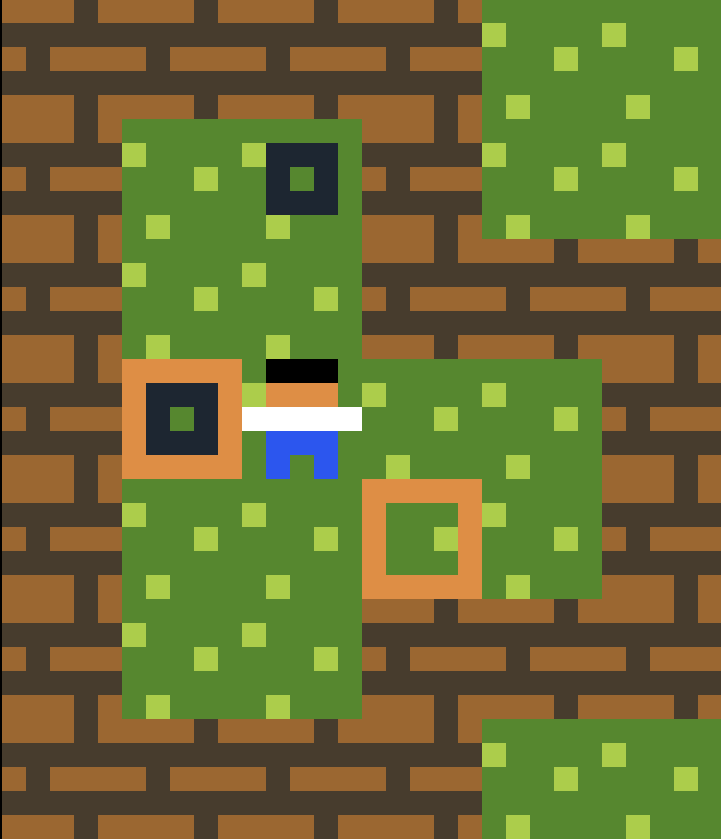
\includegraphics[width=0.7\textwidth]{figures/rulebasedimprovingfrom.png}
\end{minipage}  $\Longrightarrow$ \hfill
\begin{minipage}{0.5\textwidth}
\centering
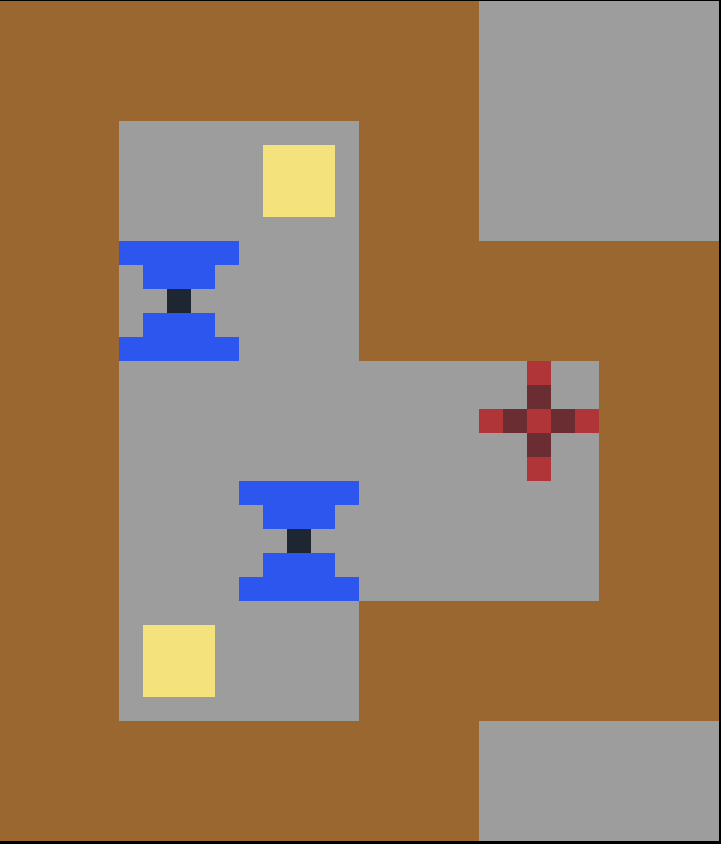
\includegraphics[width=0.7\textwidth]{figures/rulebasedimprovingto.png}
\end{minipage}
\caption{Participant 1: Mechanic swapping}
\end{figure}

% Show increpares level that looked like a classical sokoban level

\item[Gauging completeness] During the iterative design process participant 6 mentioned that he found the suggestions to be a useful stopping criterion. As soon as the suggestions did not improve the level in surprising ways, he would feel confident enough to stop iterating on the level further.

\textit{\say{Yes, especially as a level of confidence, so I was sure that the current design was pretty solid when the suggestions seemed worse.}}
\end{description}

\subsection{Adapting to the transformer}
% why that is good, why there is not 'one-design method', only one of many such tools 
Every participant did, to some degree, modify their approach towards designing puzzle levels to incorporate the transformer. While our main focus was on how we can support the user in their design process of designing puzzle levels, some participants changed their approach towards designing puzzle levels significantly in order to exploit the strengths of the transformer.

We saw a clear difference in the perceived usefulness of the tool depending on which role the tool took in the design process.

Take as an example participant 5's approach when designing puzzle levels: \\
\hspace{\dimexpr-\fboxrule-\fboxsep\relax}\fbox{%
\begin{minipage}{\textwidth}
Participant 5 first decided that his Sokoban design should be created from an empty but large field. From there, he placed a few crates and walls but quickly noticed that the tool did not find interesting transformations. This was partially because our initial settings of the transformer only added a few walls on average making almost all levels trivial but requiring much pushing around (making the solver believe that the level is difficult).

He then added more crates and targets believing that it would relinquish this error, but now the complexity of solving a single transformed level was upwards of 20 seconds.

Thinking that it takes too long to solve a single instance of a level he then added walls around the level, which should have helped to reduce the time it took to solve a single transformed level but this allowed for more unsolvable levels which were difficult to prove unsolvable.

Lastly, he manually added a wall on the top of the level, making the level significantly more difficult to his surprise.
\end{minipage}
}


Participant 5 tried to fit the tool into his method of designing puzzle games. In the beginning, he decided he would make a large Sokoban level with many crates and reluctantly changed his plans after realizing that the tool did not do so well with these kinds of levels.

Participant 1 meanwhile had a few ideas at what MixedAim might be good at and tried to find the most interesting interactions with the tool and thus did not mind changing his approach towards designing puzzle levels.

The other participants fell somewhere in between, participants 2,3,6 \& 7 used MixedAim mostly in the way we intended it to be used and did not have to significantly adapt their design approach while using the tool. Participant 4 also tried to fit the tool in his method of designing puzzle games but with success, see the backward design section for more.

These different ways of adapting to mixed-initiative tools have also been mentioned by \cite{Guzdial}, who identified a few types of participants themselves.
One group of their participants attempted to fit every suggestion their AI made into a level, something we did not encounter, and other groups of participants who adapted their behavior to discover how best to interact with the tool, similarly to participant 1.

\begin{figure}[!htbp]
\centering
\begin{minipage}[t]{0.25\textwidth}
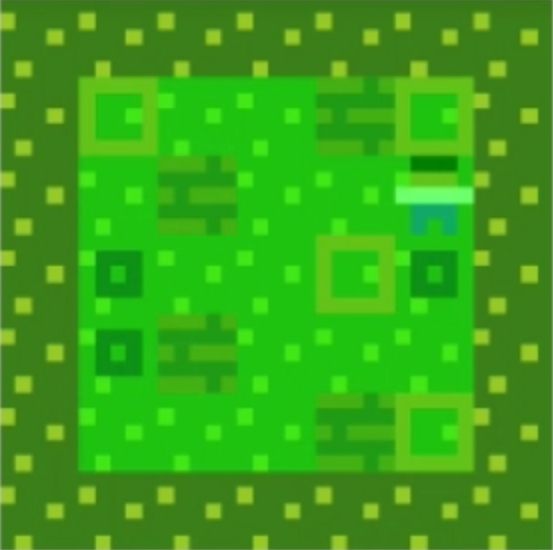
\includegraphics[width=\textwidth]{figures/part5i1_cropped.png} \hfill \\
\end{minipage}
$\Longrightarrow$
\begin{minipage}[t]{0.25\textwidth}
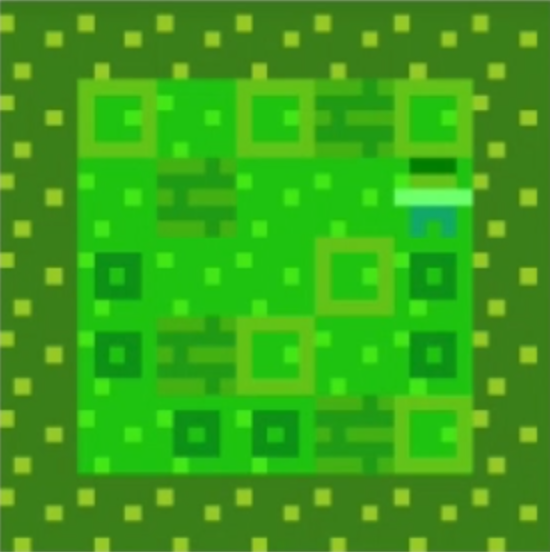
\includegraphics[width=\textwidth]{figures/part5i2_cropped.png} \hfill \\
\end{minipage}
$\Longrightarrow$
\begin{minipage}[t]{0.25\textwidth}
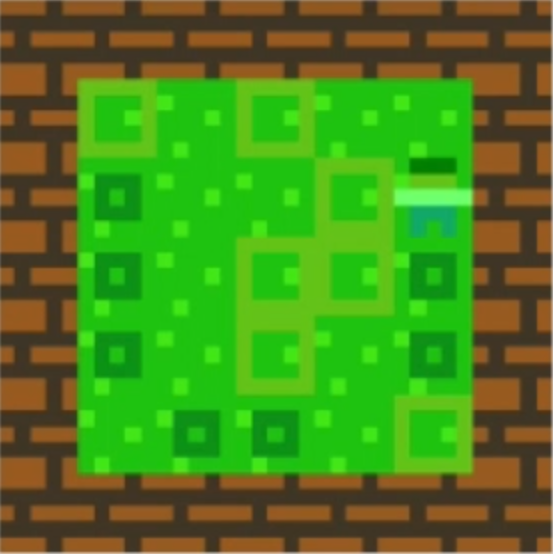
\includegraphics[width=\textwidth]{figures/part5i3_cropped.png} \hfill \\
\end{minipage}
$\Longrightarrow$
\begin{minipage}[t]{0.25\textwidth}
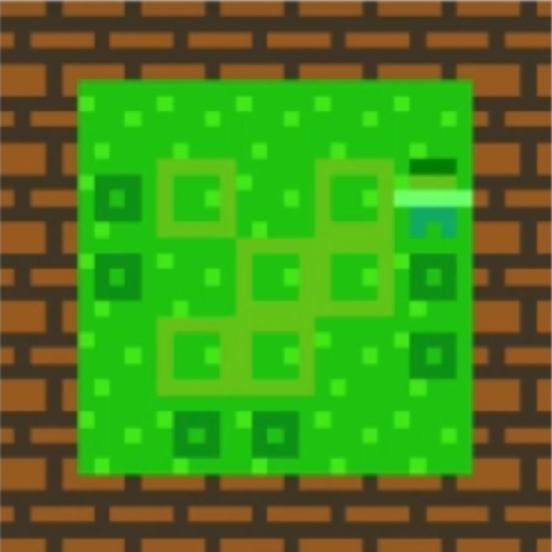
\includegraphics[width=\textwidth]{figures/part5i4_cropped.png} \hfill \\
\end{minipage}
$\Longrightarrow$
\begin{minipage}[t]{0.25\textwidth}
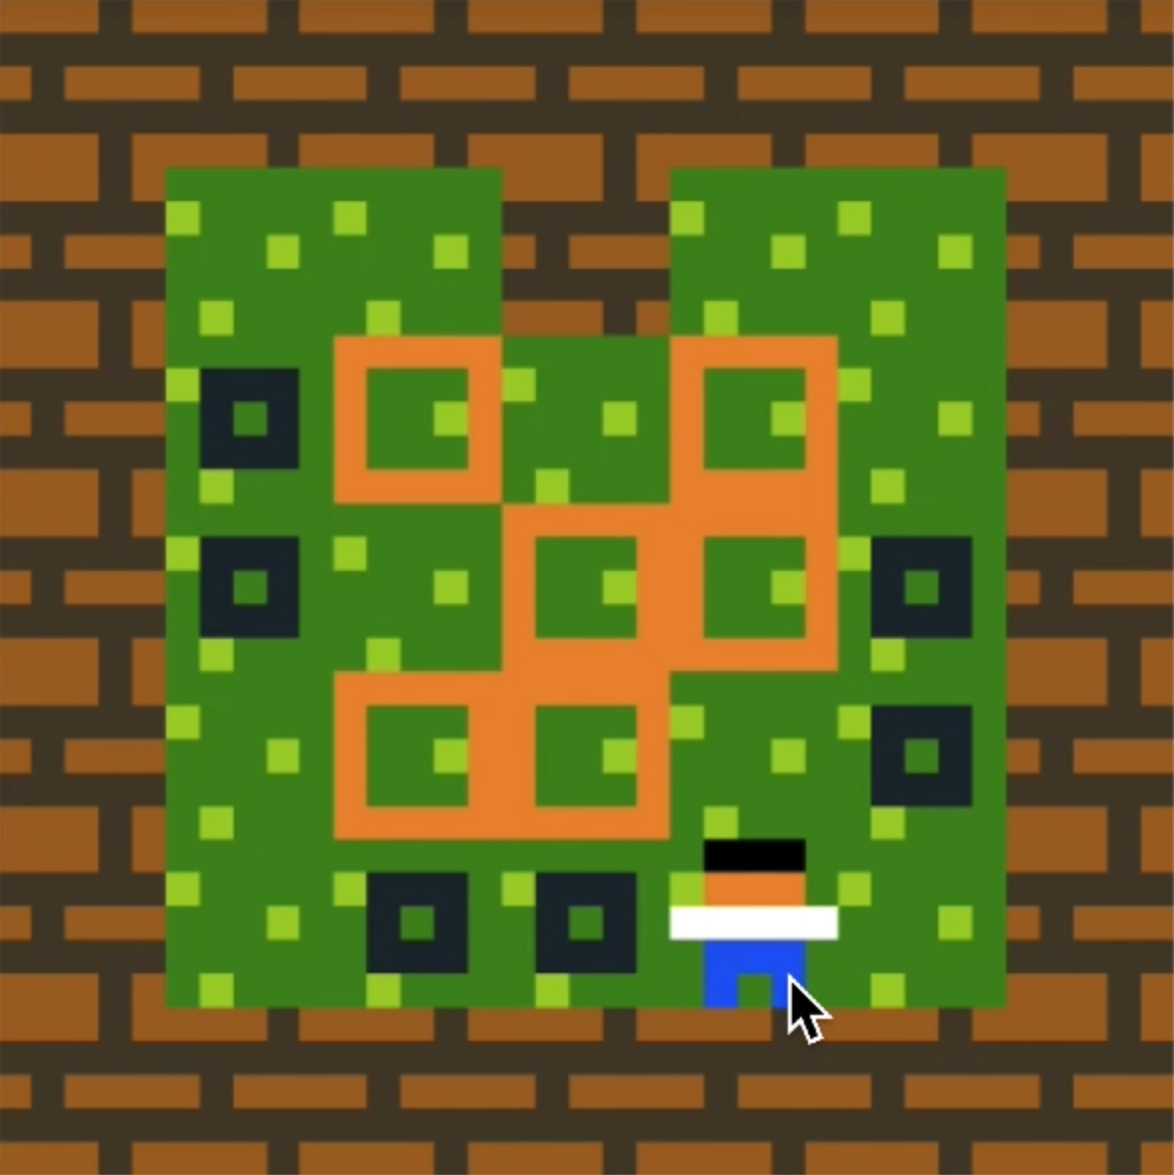
\includegraphics[width=\textwidth]{figures/part5i5.png} \hfill \\
\end{minipage}
\caption{Participant 5: Adaptive design process}
\end{figure}


We identified the following adaptions in the way users designed levels and provide a measure for judging the usefulness of an adaption based on one of these findings.


% \textbf{SUGGEST TO DISPLAY THESE FACTORS WHILE DESIGNING!!!!}



%We believe this might be because more experienced developers either tried to fit their method onto the tool (with varying degrees of success) or started to simply play around with the tool to exploit all the possible ways of creating levels.

% Under this model, we also suggest a testable hypothesis to test exotic transformers. In the end, we attempt to show a few rules of thumb that make it easy for the designer to implement such rules.



\begin{description}

    \item[Threshold-based searching] 
%Participant 1 \& 2 primarily used the transformer to identify exciting mechanics.
Participant 1 mentioned that there is a \textit{threshold} in the difficulty scores starting from which the levels become \textit{interesting}. This made him quickly change the level or the transformation rules until interesting suggestions appeared. As soon as they did, he then waited for more suggestions to appear.

\textit{\say{[...] there seems to be a threshold starting from which the levels get interesting, at least that's how it feels like qualitatively.}}

The other participants, though not stating this explicitly, acted similarly, swiftly changing the transformation rules until interesting levels occurred. When they occurred, they waited for more. For example, participant 5 frequently mentioned that the levels do not look difficult and quickly changed the transformation rules or the level until good suggestions came along.

    This threshold is entirely dependent on the level as the difficulty does not always correlate well with the perceived difficulty of the designer, something which was frequently mentioned (see negative feedback section). Sometimes this threshold is not reached due to it being difficult to solve the levels in time or because no interesting levels exist in the transformations but as soon as the threshold is reached practically all the levels are interesting.    

    With this insight we can model the usefulness of a transformation as the throughput of levels above this difficulty threshold.
\begin{equation}
\text{usefulness of transformation} = \frac{1}{\text{avg. time for interesting level}}
\label{eq:transformationusefulness}
\end{equation}
    
\begin{equation}
\text{avg. time for interesting level} = \left(1 - \frac{\text{\# interesting/difficult transformed levels}}{\text{\# total transformed levels}} \right) \cdot \text{avg. solve time}
\label{eq:transformationusefulness}
\end{equation}

    \item[Freezing sections] Participant 3 and 5 (among others) have chosen to freeze a few sections in the level, not because they necessarily thought they found these sections interesting, but to skew the search space to contain more interesting levels. For example participant 3 said quote \textit{\say{let me help it a little}} when he froze parts of the transformer section, see figure \ref{fig:part3shelp}.
    
    This adaption increases the throughput by increasing $\frac{\text{\# interesting difficult transformed levels}}{\text{\# total transformed levels}}$.
        
\begin{figure}
\centering
\begin{minipage}[t]{0.3\textwidth}
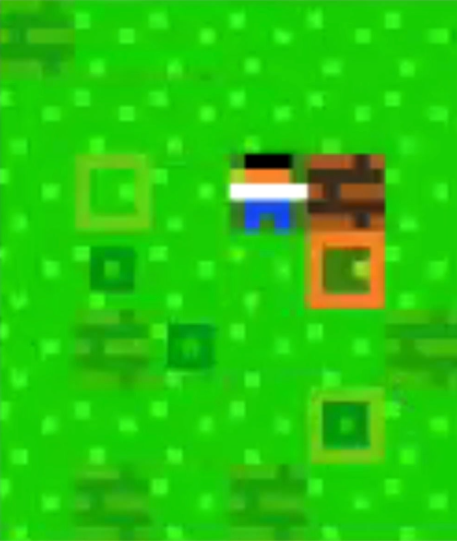
\includegraphics[width=\textwidth]{figures/part3helpalittlefrom.png} \\
\end{minipage}
$\Longrightarrow$
\begin{minipage}[t]{0.3\textwidth}
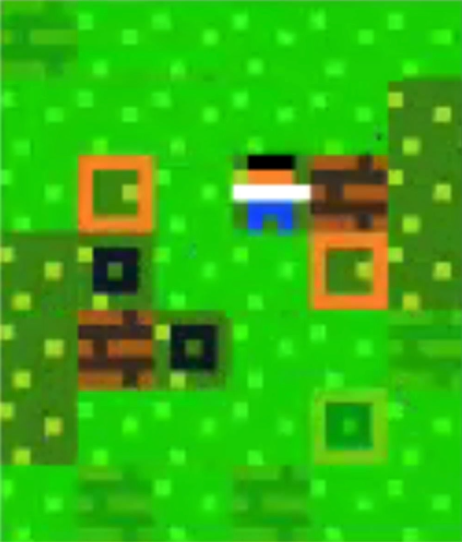
\includegraphics[width=\textwidth]{figures/part3helpalittleto.png} \\
\end{minipage}
\caption{Participant 3 freezing sections to aid the transformer\label{fig:part3shelp}}
\end{figure}

    
    \item[Smaller levels] Participant 1 concluded that the transformer is well-suited to create small Sokoban levels, see figure \ref{fig:part1smallsokoban}. He also experimented with variations of Sokoban rules and created a few puzzle games with small levels using this method (\href{https://www.increpare.com/game/all-green-to-blue.html}{'All Green To Blue'}\footnote{\url{https://www.increpare.com/game/all-green-to-blue.html}} and \href{https://www.increpare.com/game/all-green-and-blue-on-yellow.html}{'All Green To Blue On Yellow'}\footnote{\url{https://www.increpare.com/game/all-green-and-blue-on-yellow.html}} which are playable online), see  \autoref{fig:part1smalllevelgames}.
    
    This adaption increases the throughput by increasing the \textit{average time for solving a transformed level}.
    
    
    \begin{figure}
\centering
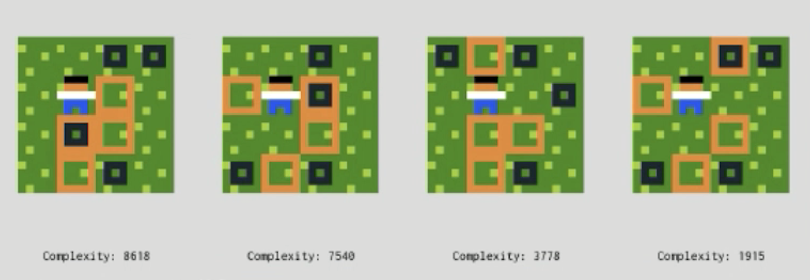
\includegraphics[width=\textwidth]{figures/part1_smallsokobandesigns.png}
\caption{Participant 1's small Sokoban transformations \label{fig:part1smallsokoban}}
\end{figure}


\begin{figure}
\centering
\begin{minipage}[t]{0.3\textwidth}
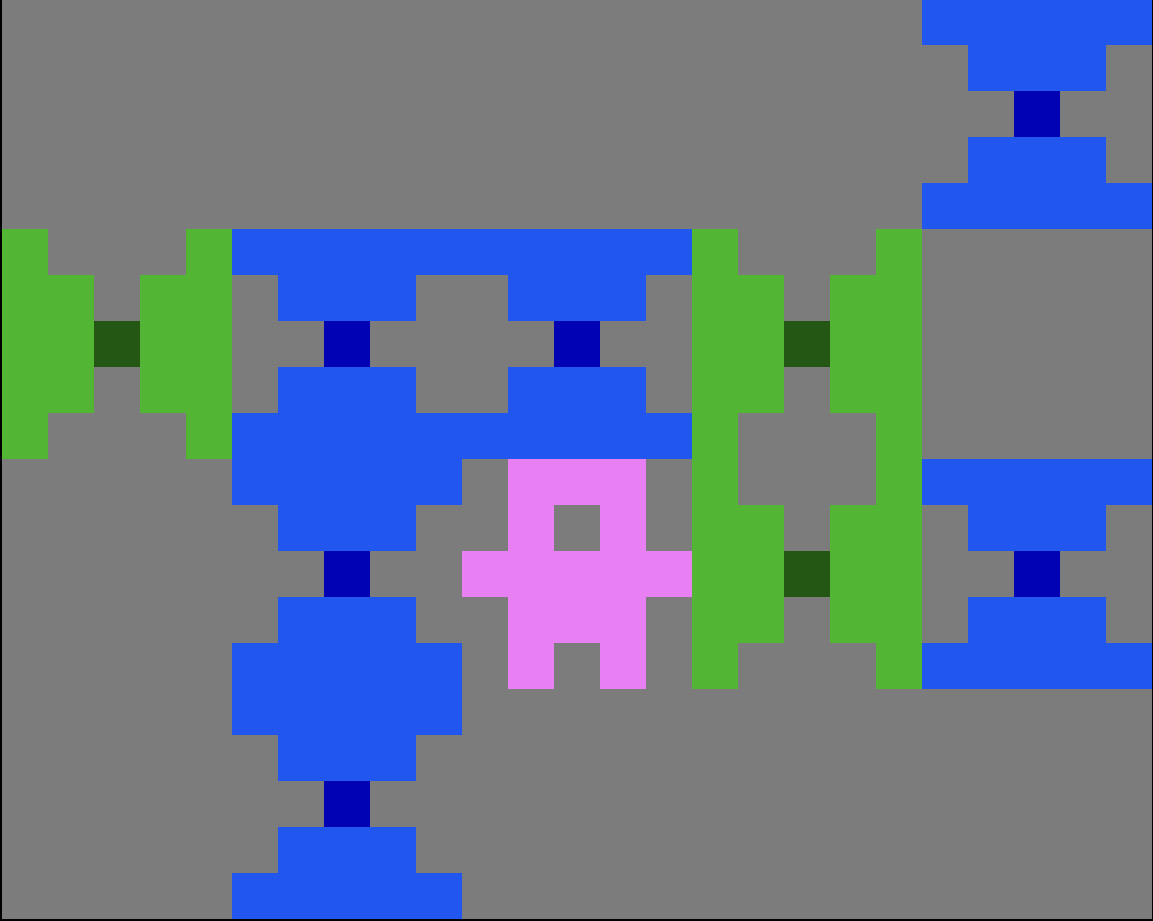
\includegraphics[width=\textwidth]{figures/part1AllGreenToBlue.png} \\
\end{minipage}

\begin{minipage}[t]{0.3\textwidth}
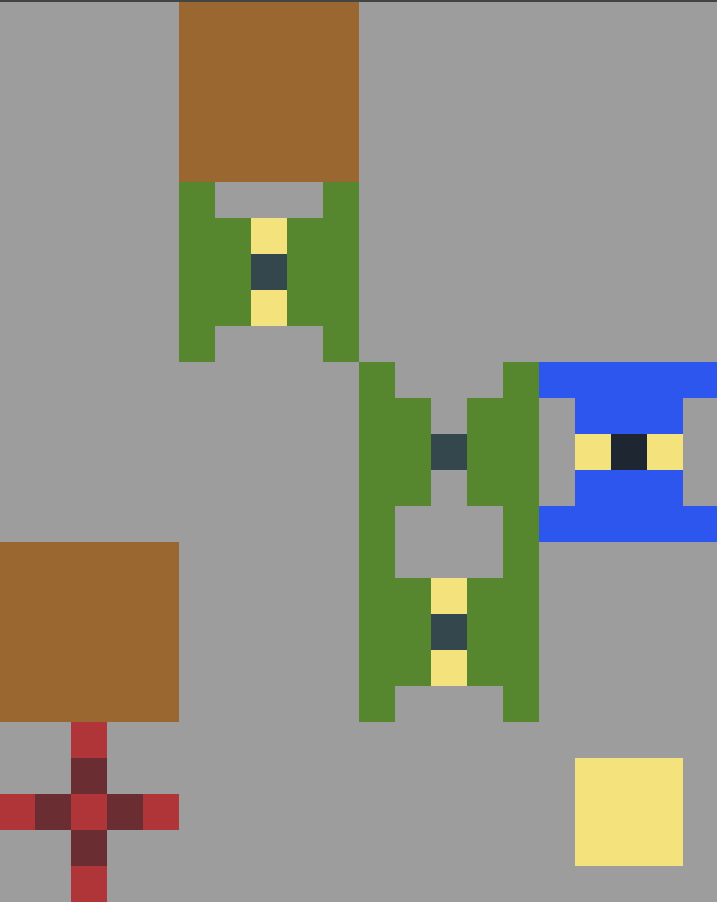
\includegraphics[width=\textwidth]{figures/part1allgreentoblueonyellow.png} \\
\end{minipage}
\caption{Participant 1's custom games \label{fig:part1smalllevelgames}}
\end{figure}

    \item[Larger levels] Participant 5 decided that larger levels would be better for the transformer because it would allow for a larger quantity of interesting levels. However, this approach also allows for more uninteresting levels and significantly decreased the \textit{average time for solving a transformed level}, which made choosing larger levels a bad adaption to the system.
    
    \item[More variation] Lastly, we observed that some games are better suited for identifying interesting mechanics than others. Both we and participant 2 have had such success with puzzle games that feature polyominoes.

This leads us to believe that Sokoban-like puzzle games with a lot of possible variations in a small space are especially well-suited for identifying interesting mechanics. When focusing on small levels it does not take a lot of time to find a solution or prove that no solution exists and would take at most in the order of $\mathcal{O}\left( {n^2 \choose a} \right)$ computational steps, where $a$ are the number of blocks in the generated level and $n^2$ are the possible places the blocks can be placed. Notice that using a variety of different objects (for example differently shaped polyominoes) does not change the value of $a$. Thus one can build more interesting small levels with puzzle games that have a lot of different types and shapes of objects, as opposed to games with only three types of $1 \times 1$ objects. 

% \item[Structural changes] 


\end{description}

\subsection{Backward designing}

\begin{figure}
\centering
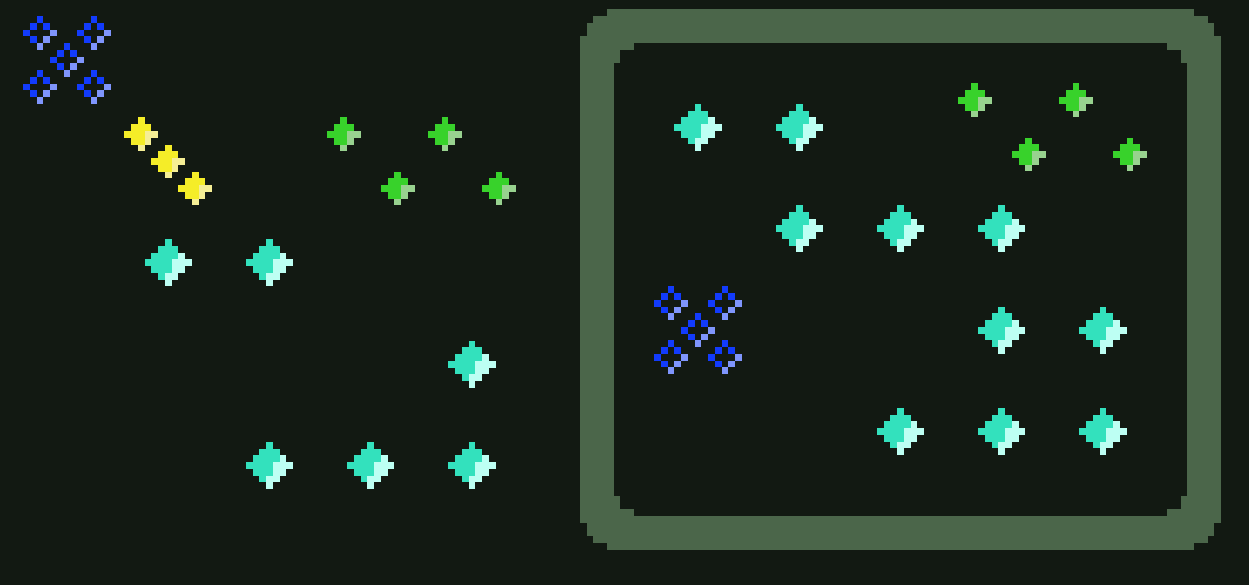
\includegraphics[width=.85\textwidth]{figures/backward_design_minotalen.png}
\caption{Backward design of participant 4's puzzle game\label{fig:backwarddesign}}
\end{figure}

This method of designing levels with the mixed-initiative system was discovered and coined by participant 4 and was not an approach of designing puzzles with MixedAim we had foreseen. In backward design, one starts to design a level from a solved state and slowly turns it into a more complicated/interesting, but always solvable, level.
Participant 4 used it specifically for their PuzzleScript game \ref{fig:backwarddesign} but this backward approach can also be used for Sokoban. 

% Participant 4 used it on a block expanding level 

Both \cite{Taylor2011} and \cite{Kartal2015} have employed such a backward design approach for generating Sokoban levels. We will now illustrate how their approaches can be formulated as transformer rules in MixedAim with which designers could interactively backward design.

\begin{description}
\item[\cite{Taylor2011}] This assumes that the target positions are fixed and no crates are in the initial design. The player then pulls the crates away from the goal.
\begin{lstlisting}
(place crates on all targets)
[Target No Crate] -> [Target Crate]
(move the player around and let him pull crates)
choose 50 [Player | No Obstacle] -> [| Player]
or [No Obstacle | Player | Crate] -> [Player | Crate | ]    
\end{lstlisting}

\item[\cite{Kartal2015}] This assumes that the crate positions are fixed and no targets are in the initial design. The player then pushes the crates around and at the end turns them into targets.

\begin{lstlisting}
(add a placeholder to all crates)
[Crate] -> [Crate Placeholder]
(move the player around and let him push crates)
choose 50 [Player | No Obstacle] -> [ | Player]
or [Player | Crate | No Obstacle] -> [ | Player | Crate] 
(replace crates with targets and placeholders with crates)
[Crate] -> [Target]
[Placeholder] -> [Crate]
\end{lstlisting}
\end{description}

\section{Structured Interview Responses}

For most participants, we took the structured interview immediately after the think-aloud study, depending on the preference in writing or orally. Participants 1 and 4 did the structured interview after using the tool for a few days testing it not only on Sokoban but also on their games. Since the questions are quite open-ended, we would skip a few of them if the participant had already answered them in a previous question. 

We compiled a list of the most interesting answers to the questions in the appendix \autoref{apx:interview} but believe that the most important insights from the interviews have either been mentioned or are elaborated in the next sections.



\section{Negative feedback}

Unfortunately, not all participants had a very smooth experience with the tool. Especially participant 5 immediately decided that interesting Sokoban levels were large and would contain many crates which unfortunately the transformer did not handle very well. The designer then had to limit himself to designs which the transformer handled better.

He also admitted that while making levels with the tool can be more efficient, passively showing information can take the fun out of solving the level and one might be easily tempted to look at the solution instead of working it out in the head \ref{fig:part5comments}.

Participant 6 addressed the same concern mentioning that there is a `Google effect' that makes him stop thinking about solvability (Google effect meaning that people do not attempt to remember a fact but instead remember how to look it up instead). He did not see this in a negative light though, and enjoyed that it made the process faster.

\begin{figure}
\begin{minipage}[t]{\textwidth}
\textit{\say{Part of designing a puzzle is trying to make the best puzzle you can make, but part of it is also the fun of solving intermediate states yourself. So that's one thing that I would miss with the software (you might be able to work around it) but one thing I like about designing puzzles, is to constantly be thinking about solutions in my head, so this is kind of giving this up a little bit, and I'm not actively thinking about solutions when I'm designing.}} \hfill \\

\textit{\say{I can create better puzzles with this tool but might have less fun while doing it.}}

\textit{\say{There's a kind of Google effect where I stop thinking about solvability.}}

\end{minipage}
\caption{Participant 5 \& 6's quotes regarding solvability\label{fig:part5comments}}
\end{figure}



Participant 1, who is very experienced with puzzle design, has a different mindset towards the transformer and thinks that it adds another tool for inventing levels.

Participant 1 fears that designers who have not had much manual puzzle-developing experience would end up making uninteresting levels, which are just `interesting enough' to put into a game. \cite{Guzdial} mentioned similar concerns that their tool could replicate an over-used design. This gives an additional responsibility to the designer, who now has to resist relying too much on the system.

Participant 1's quote sums it up nicely: 
\textit{\say{They're cool to work with [referencing the tools], but it's so easy to make bad and difficult levels (a fatal combo).}} % from tweet

\section{Suggestions}

\begin{description}
    \item[Use more sophisticated curators / more accurate difficulty measure]
A very common complaint (every participant except for 1, 5 and 6 mentioned it) was that we curated levels based only on the difficulty of the solver and that the difficulty of the solver also does not always match the perceived difficulty.

\textit{\say{The limitations are [the systems] judging abilities.} -- Participant 3}

Due to time constraints, we decided from the beginning to keep the curator very simple. However, after interviewing participant 1 \& 4 we have a suggestion for future work to improve upon the curator. We suggest adding an optional `cost' modifier to operational rules. 

 For example: \lstinline{[ > Player | Crate ] -> [ > Player | > Crate ] COST 10} \hfill \\
 This way, levels that require more costly rules in order to be solved are given a higher difficulty score. The rule above would discourage levels that need a lot of moving around without pushing blocks.

% more pushing of blocks are weighted more and gives control to the designer and lets him implement their subjective experience of what makes a difficult puzzle game.
 

    \item[Feedback for adapting to the transformer]
    Participant 4 suggested showing how many levels have already been transformed to get an estimate of the effectiveness of the transformer.
    
    We suggest to take this a step further and also show the throughput of curated levels and also show how many levels are solvable/unsolvable/timed-out, respectively. These changes would allow the user to better adapt their actions towards the transformer. 
    
    \item[Unresponsiveness]
    Many participants felt like the transformer was unresponsive at times, due to there being no visual feedback when MixedAim found no suitable suggestions. Participant 4 \& 7 both suggested adding a button to explicitly generate the levels instead of automatically transforming them, while Participant 1 suggested labeling more clearly that the transformer was doing its work.
    
    \item[Improve UI] A suggestion by participant 5 was that the tool should have an option to enable/disable showing passive information about a level since knowing that a solution exists can tempt you to click on it instead of solving it yourself, which is an aspect he would otherwise miss when designing puzzle games.
     
     \item[Level progression aid] Participant 4 suggested that the tool should also help with creating an engaging level progression sequence. This is far beyond the scope of our work. However, \cite{Butler2013} has promising work in this direction. 
    
\end{description}

\section{Conclusion}

We developed the mixed-initiative system MixedAim for creating PuzzleScript games interactively with the computer. For this purpose we generalized the Sokoban heuristic of \cite{Jurgen} to solve levels more efficiently, we crafted a user interface which supported various forms of direct manipulation, like using a level editor and play-testing the level and added support for interactive suggestions. We hypothesized and later confirmed that giving more difficult suggestions is a feasible way to assist the designer. Specifically, we have identified that there is a threshold in difficulty starting from which levels become interesting.

We identified various key interactions with those suggestions that designers and illustrated in which way designers could benefit from them. Interactions included \textit{Identifying and constraining mechanics and aesthetics in designs}, \textit{making unsolvable levels work again through transforming},  \textit{window dressing}, \textit{mechanic swapping}, \textit{gauging completeness} and \textit{backward designing}.

Furthermore, we analyzed how participants adapted to the MixedAim suggestions, identified that the perceived usefulness is dependent on the role of MixedAim in the design process and noticed that it was particularly good at identifying interesting mechanics in small levels with a lot of possible variations.

Through the user interviews, we identified that some designers experienced a `Google effect' that made users delegate the responsibility of solving the level to the MixedAim system. Some view this as taking out the fun, while others think this is efficient. Lastly, we also received concerns that the tool can make it easy to create difficult and bad levels which give additional responsibility to the designer planning to incorporate such tools in their workflow.

Overall, we believe that mixed-initiative methods add value to the design process if they are approached as just another tool in the toolset for creating puzzle games and not as the de facto replacement of one's usual design process.
